\documentclass[11pt]{article}

% Packages
\usepackage[margin=1in, top=0.7in]{geometry}
\usepackage{amsmath,amssymb,amsfonts}
\usepackage{graphicx}
\graphicspath{{./}{../}}
\usepackage{hyperref}
\usepackage{algorithm}
\usepackage{algpseudocode}
\usepackage{booktabs}
\usepackage{longtable}
\usepackage{multirow}

% Document info
\title{Assignment 3 Report\\
    CS-726: Advanced Machine Learning}
\author{Deeptanshu Malu \quad Deevyanshu Malu \quad Neel Rambhia}
\date{}

\begin{document}

\maketitle

\section{Task 0}

The output provided on running the program is:

\begin{verbatim}
Using device: cuda

--- Model Architecture ---
EnergyRegressor(
    (net): Sequential(
        (0): Linear(in_features=784, out_features=4096, bias=True)
        (1): ReLU(inplace=True)
        (2): Linear(in_features=4096, out_features=2048, bias=True)
        (3): ReLU(inplace=True)
        (4): Linear(in_features=2048, out_features=1024, bias=True)
        (5): ReLU(inplace=True)
        (6): Linear(in_features=1024, out_features=512, bias=True)
        (7): ReLU(inplace=True)
        (8): Linear(in_features=512, out_features=256, bias=True)
        (9): ReLU(inplace=True)
        (10): Linear(in_features=256, out_features=128, bias=True)
        (11): ReLU(inplace=True)
        (12): Linear(in_features=128, out_features=64, bias=True)
        (13): ReLU(inplace=True)
        (14): Linear(in_features=64, out_features=32, bias=True)
        (15): ReLU(inplace=True)
        (16): Linear(in_features=32, out_features=16, bias=True)
        (17): ReLU(inplace=True)
        (18): Linear(in_features=16, out_features=8, bias=True)
        (19): ReLU(inplace=True)
        (20): Linear(in_features=8, out_features=4, bias=True)
        (21): ReLU(inplace=True)
        (22): Linear(in_features=4, out_features=2, bias=True)
        (23): ReLU(inplace=True)
        (24): Linear(in_features=2, out_features=1, bias=True)
    )
)
------------------------

Loading dataset from ../A4_test_data.pt...
Dataset loaded in 0.17s. Shape: x=torch.Size([100000, 784]), energy=torch.Size([100000, 1])

--- Test Results ---
Loss: 288.1554
--- Script Finished ---
\end{verbatim}

\section{Task 1}

10000 samples were taken in total using each algorithm. 2000 samples were used for burn-in and 8000 samples were used for sampling.

\begin{longtable}{|l|c|c|c|}
    \hline
    \textbf{Sampling Algorithm} & \textbf{Burn-in time (s)} & \textbf{Sampling time (s)} & \textbf{Total time (s)} \\
    \hline
    Algorithm 1 & 19.37 & 71.23 & 90.60 \\
    \hline
    Algorithm 2 & 8.19 & 32.53 & 40.72 \\
    \hline
    \caption{Performance comparison of sampling algorithms for 10,000 samples.}
\end{longtable}

\begin{figure}[H]
    \centering
    \begin{tabular}{cc}
        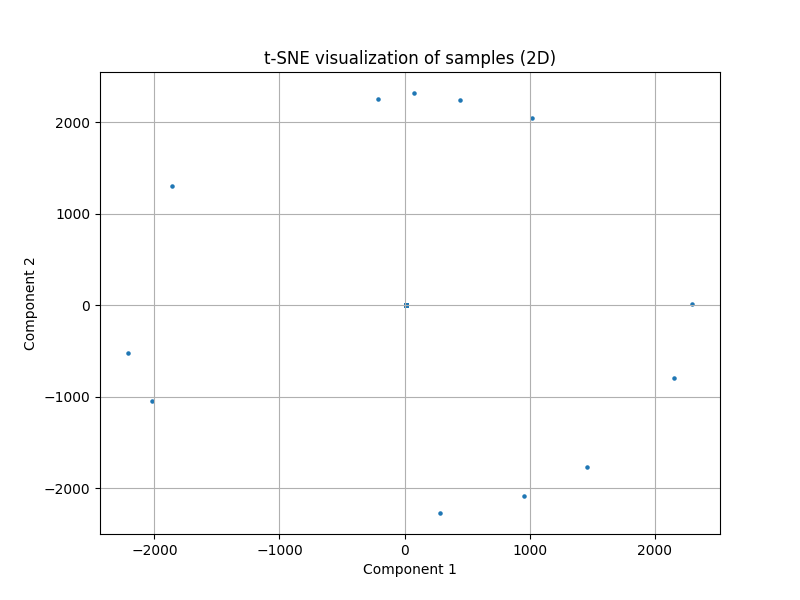
\includegraphics[width=0.4\textwidth]{../TASK-0-1/tsne_plot_sklearn_2d_1.png} &
        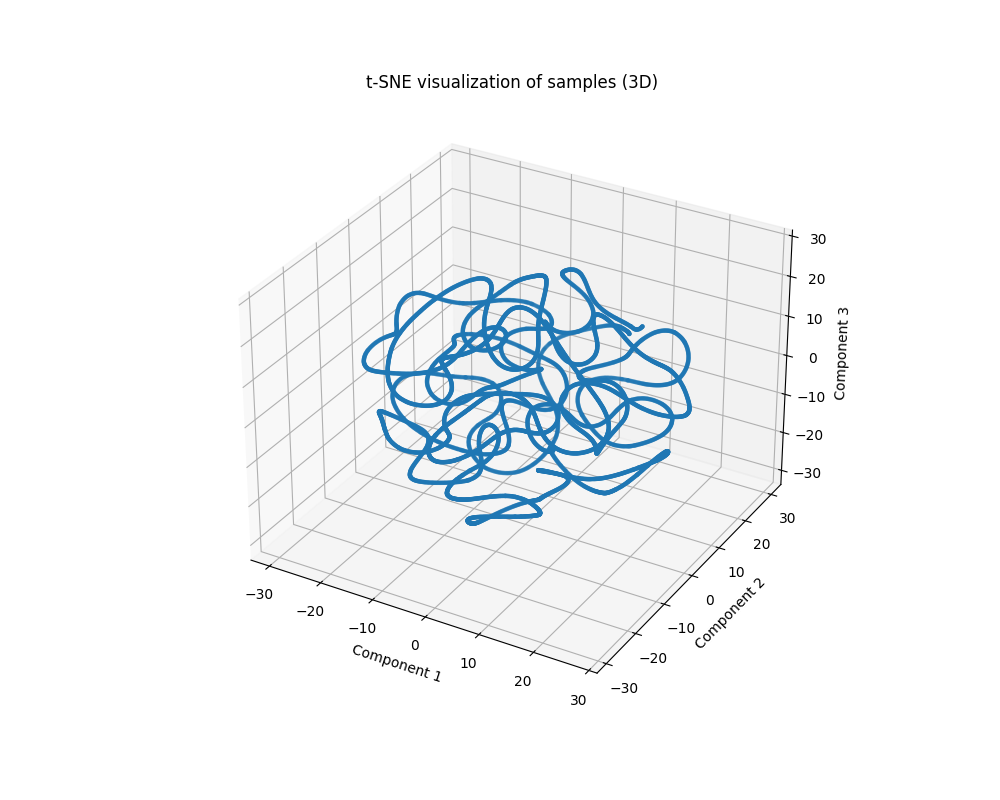
\includegraphics[width=0.4\textwidth]{../TASK-0-1/tsne_plot_sklearn_3d_1.png} \\
        Algorithm 1 t-SNE 2d & Algorithm 1 t-SNE 3d \\[0.5em]
        
        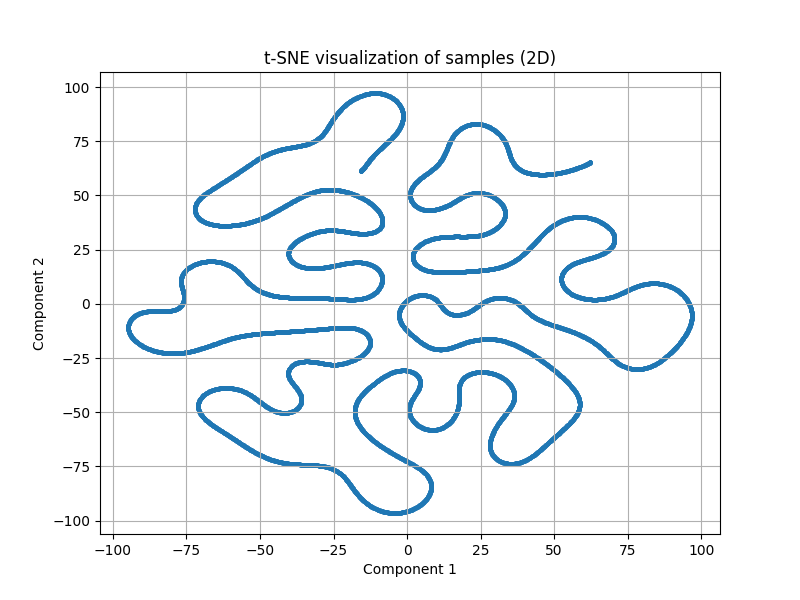
\includegraphics[width=0.4\textwidth]{../TASK-0-1/tsne_plot_sklearn_2d_2.png} &
        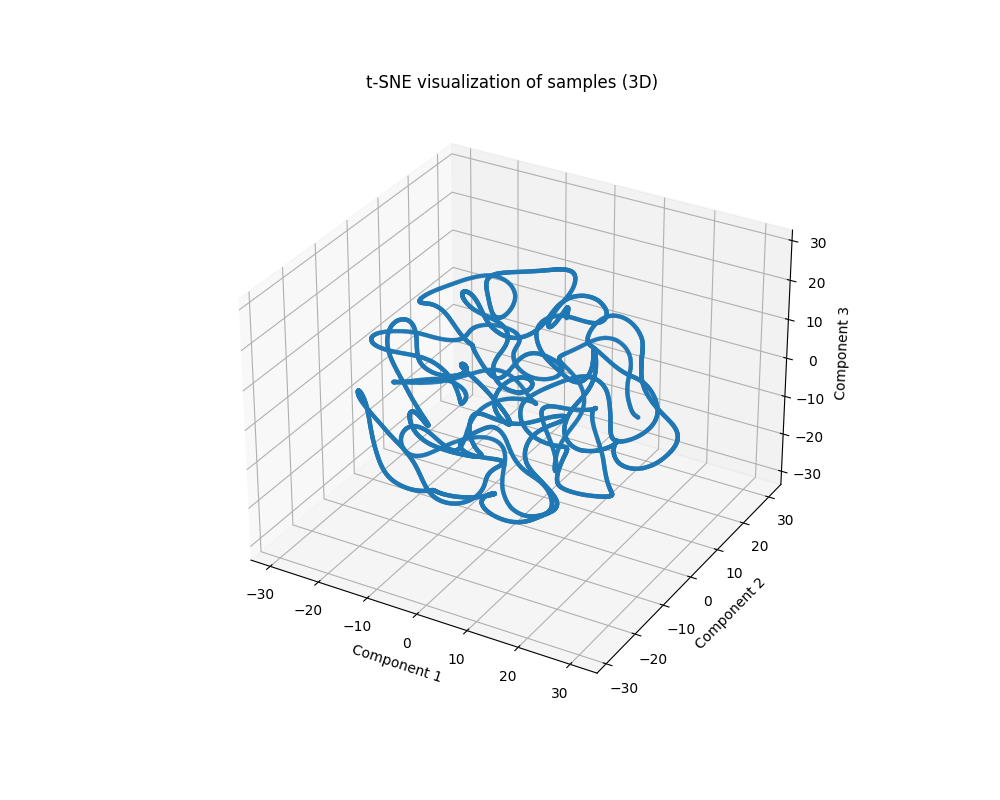
\includegraphics[width=0.4\textwidth]{../TASK-0-1/tsne_plot_sklearn_3d_2.png} \\
        Algorithm 2 t-SNE 2d & Algorithm 2 t-SNE 3d \\
    \end{tabular}
    \caption{t-SNE plots for the two sampling algorithms.}
    \label{fig:tsne}
\end{figure}

\section{Task 2}

n is the number of samples taken from the Branin-Hoo function.

\begin{figure}[H]
    \centering
    \begin{tabular}{cccc}
        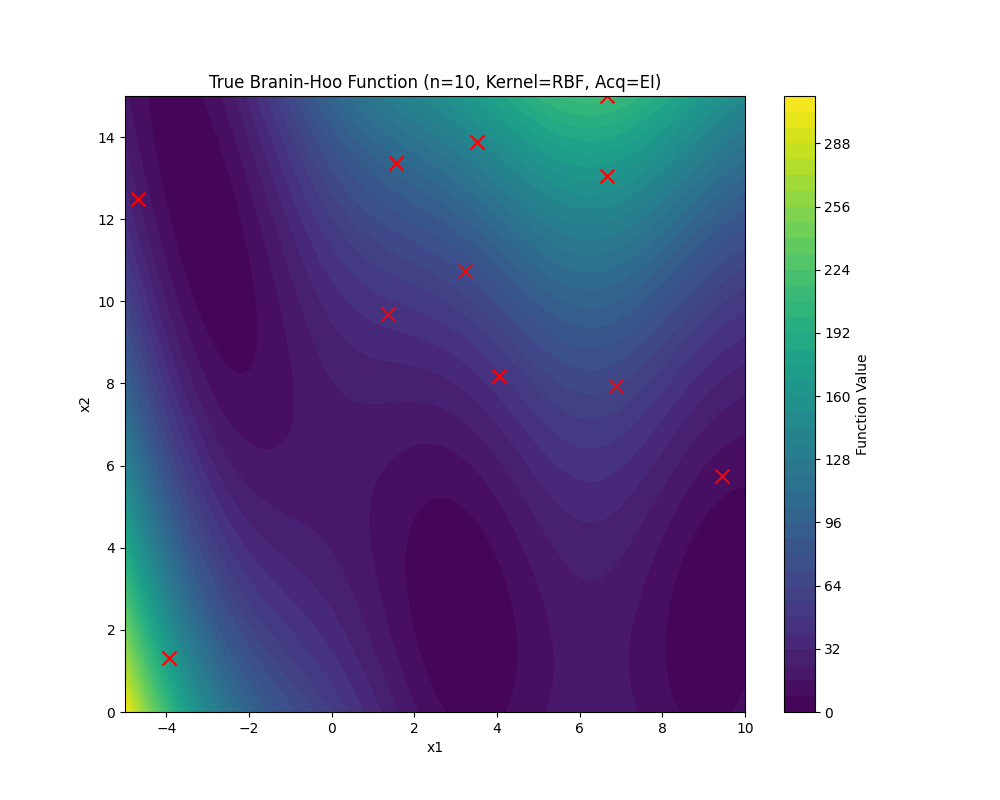
\includegraphics[width=0.225\textwidth]{../Task-02/plots/true_function_rbf_n10_EI.png} &
        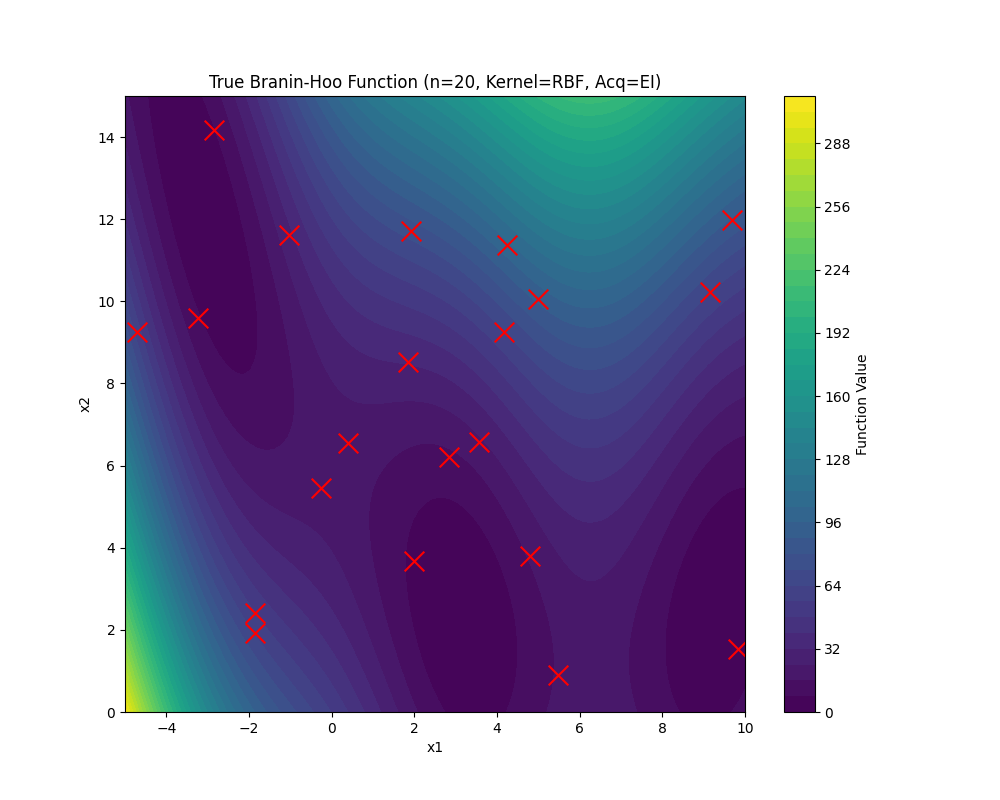
\includegraphics[width=0.225\textwidth]{../Task-02/plots/true_function_rbf_n20_EI.png} &
        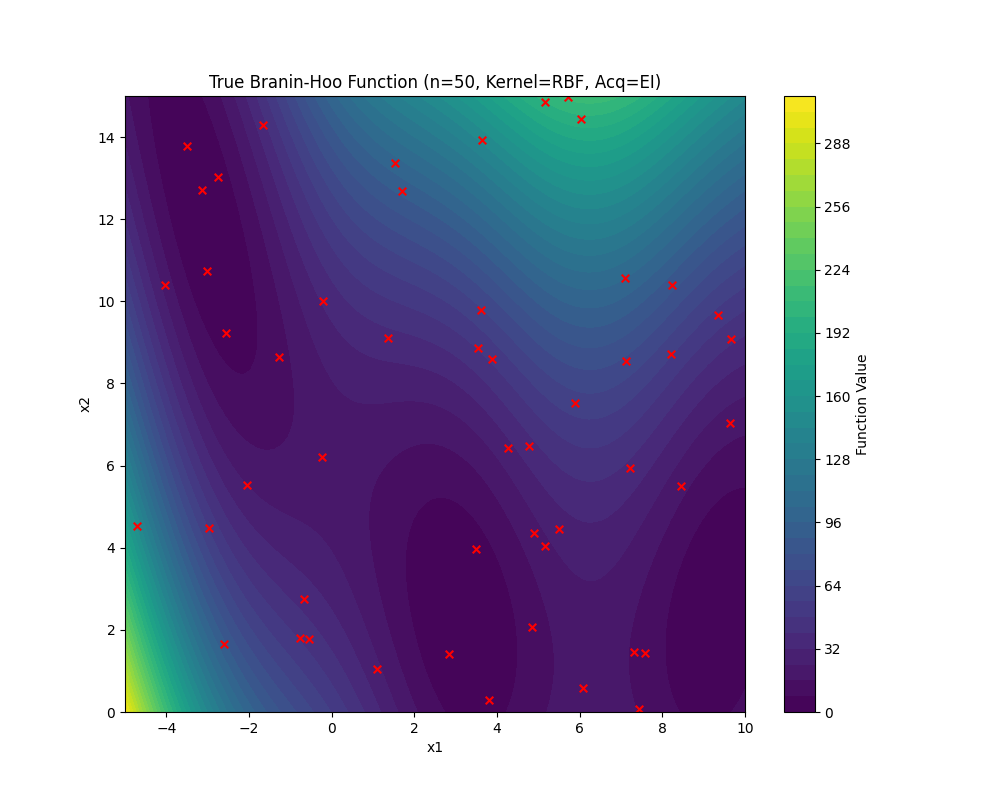
\includegraphics[width=0.225\textwidth]{../Task-02/plots/true_function_rbf_n50_EI.png} &
        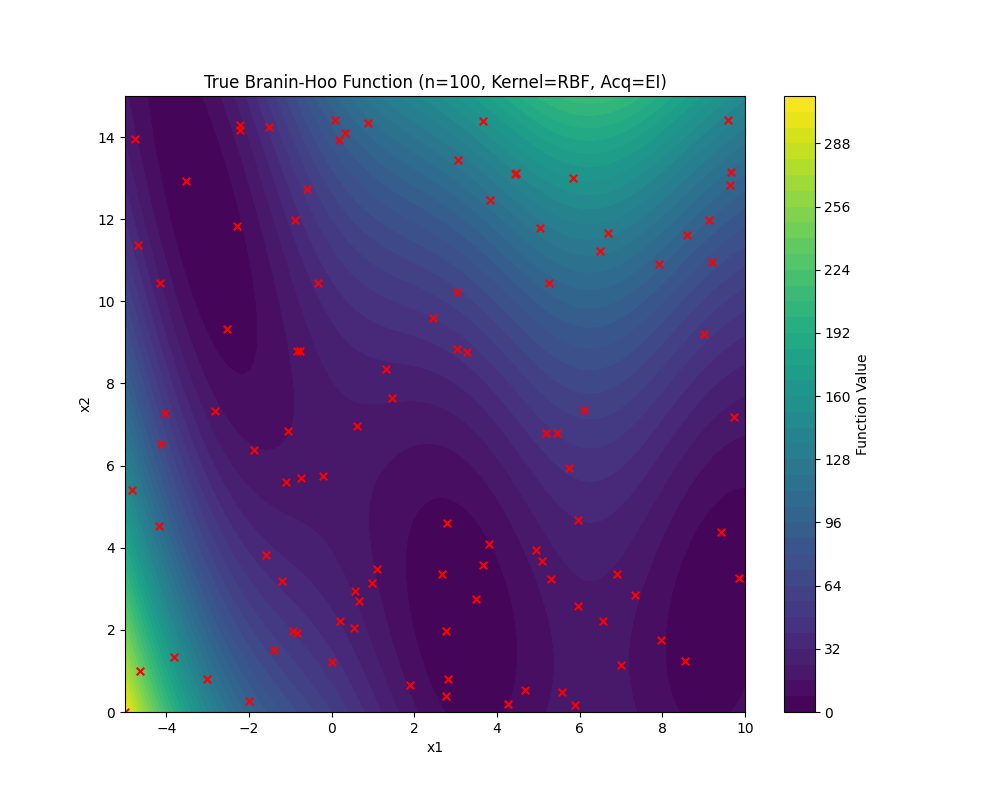
\includegraphics[width=0.225\textwidth]{../Task-02/plots/true_function_rbf_n100_EI.png} \\
        n=10 with EI & n=20 with EI & n=50 with EI & n=100 with EI \\[0.5em]
        
        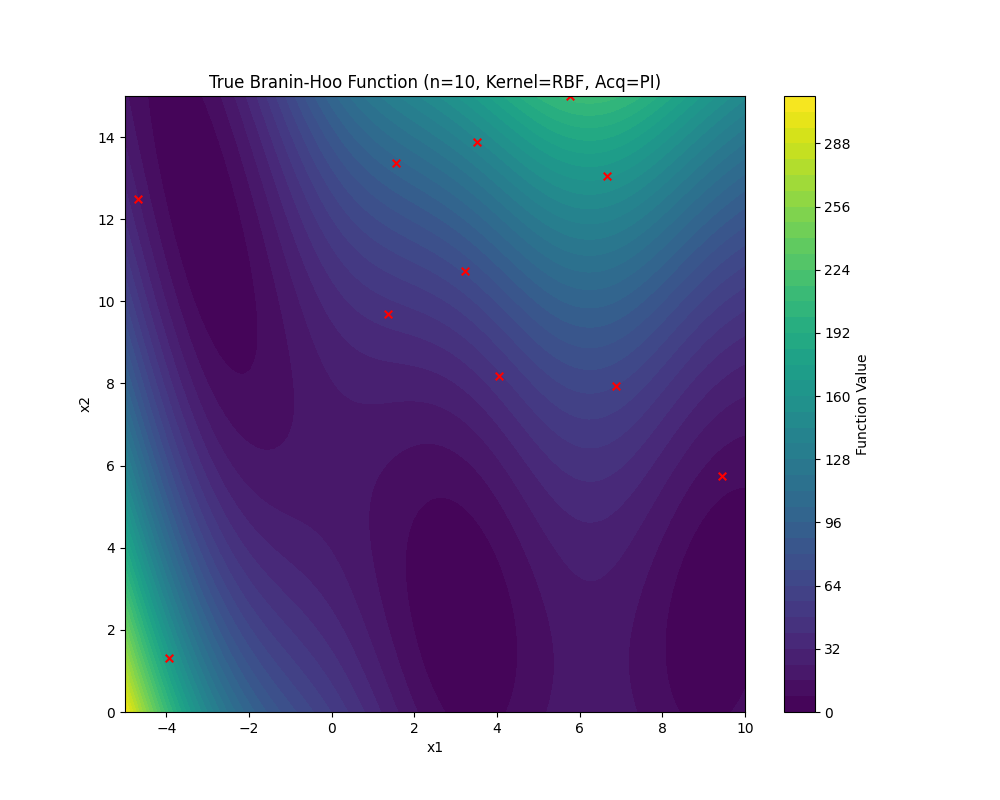
\includegraphics[width=0.225\textwidth]{../Task-02/plots/true_function_rbf_n10_PI.png} &
        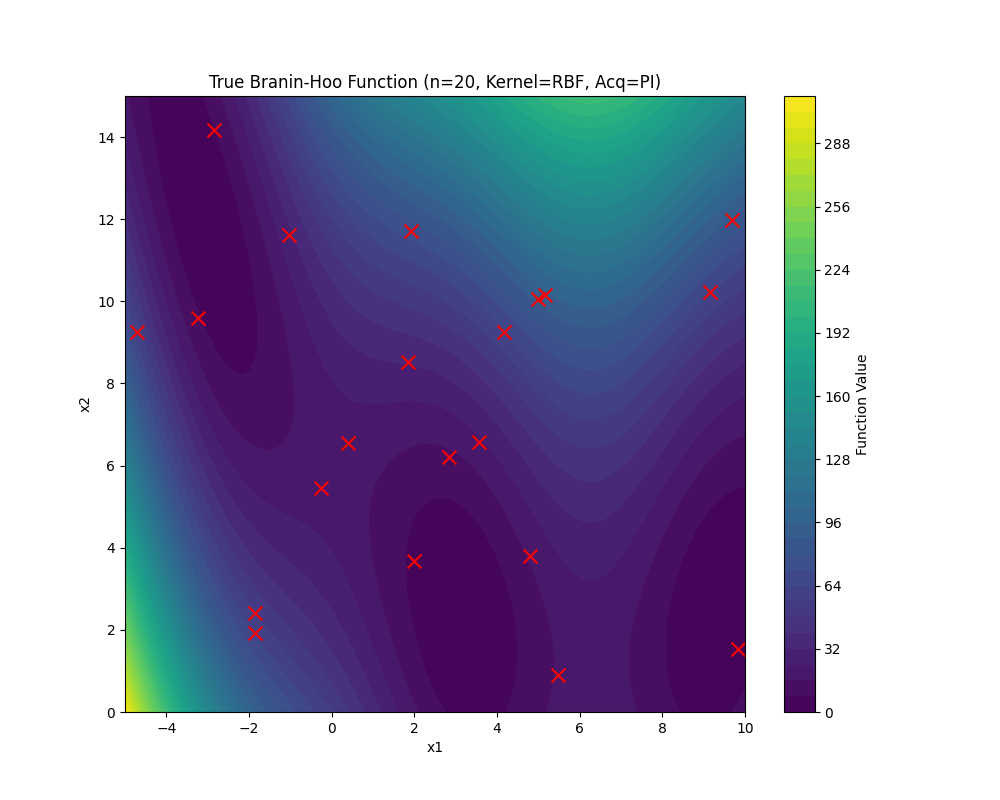
\includegraphics[width=0.225\textwidth]{../Task-02/plots/true_function_rbf_n20_PI.png} &
        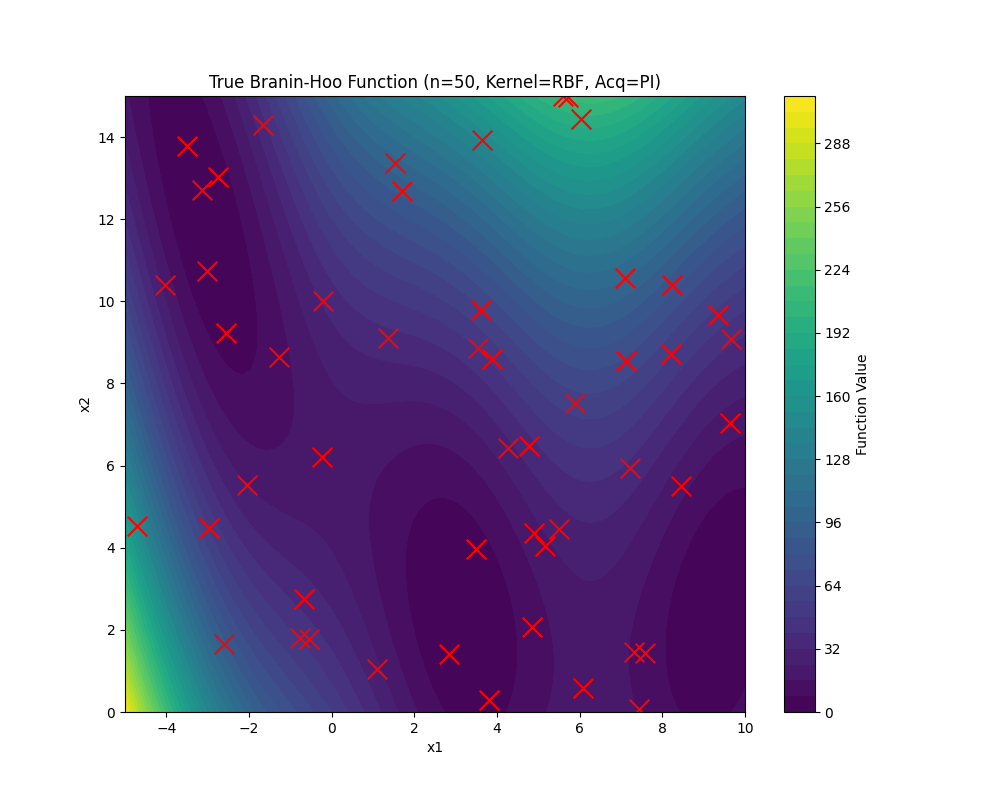
\includegraphics[width=0.225\textwidth]{../Task-02/plots/true_function_rbf_n50_PI.png} &
        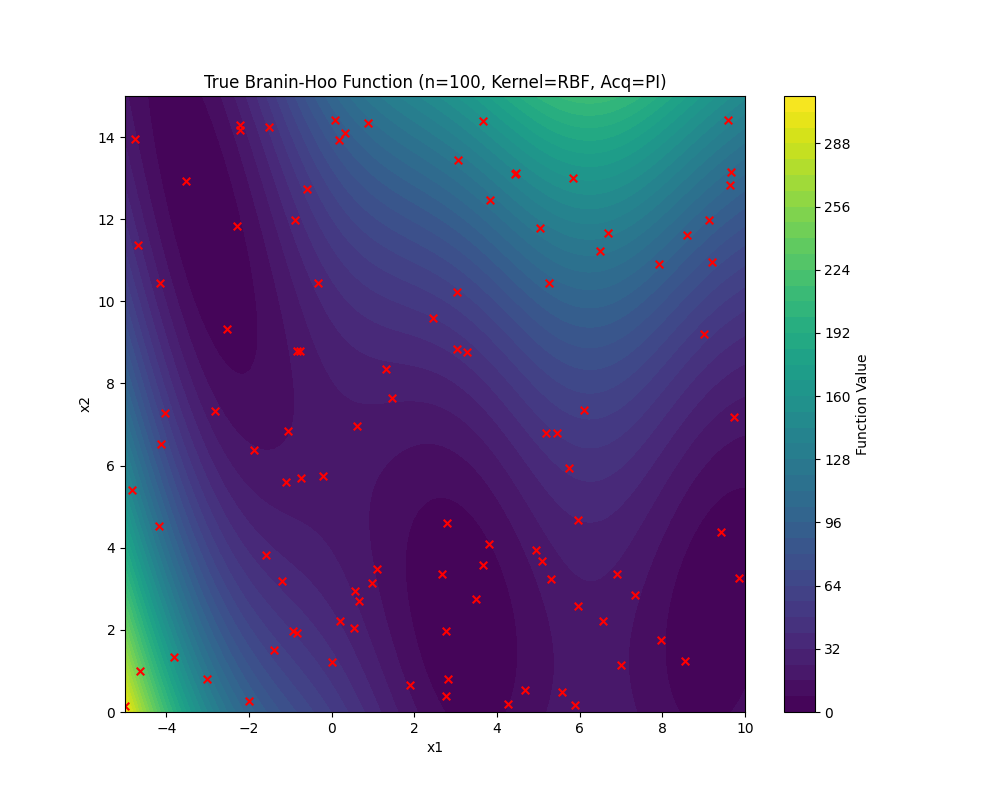
\includegraphics[width=0.225\textwidth]{../Task-02/plots/true_function_rbf_n100_PI.png} \\
        n=10 with PI & n=20 with PI & n=50 with PI & n=100 with PI \\
    \end{tabular}
    \caption{RBF kernel true function with different acquisition functions.}
    \label{fig:rbf_true_function}
\end{figure}

\begin{figure}[H]
    \centering
    \begin{tabular}{cccc}
        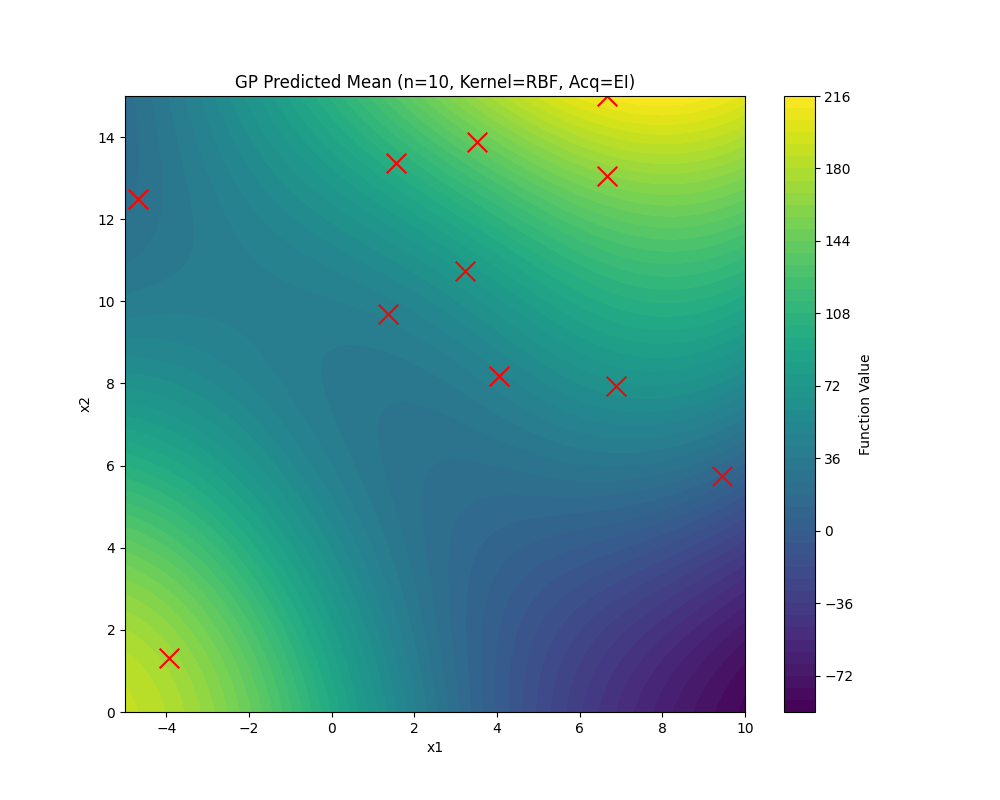
\includegraphics[width=0.225\textwidth]{../Task-02/plots/gp_mean_rbf_n10_EI.png} &
        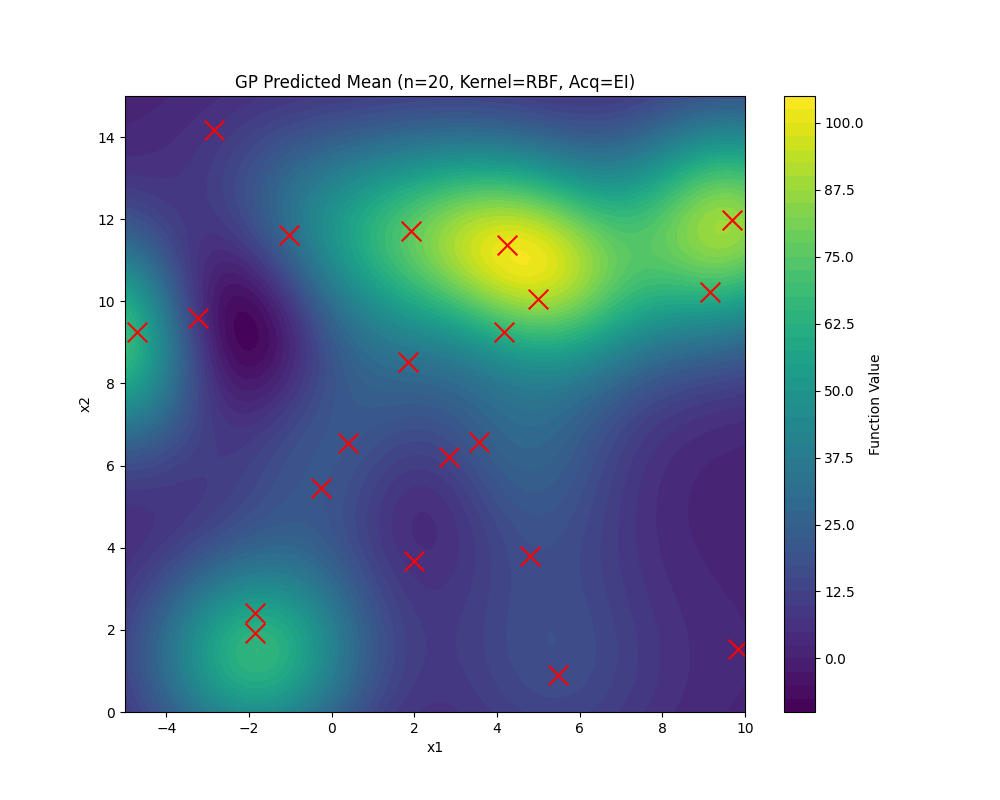
\includegraphics[width=0.225\textwidth]{../Task-02/plots/gp_mean_rbf_n20_EI.png} &
        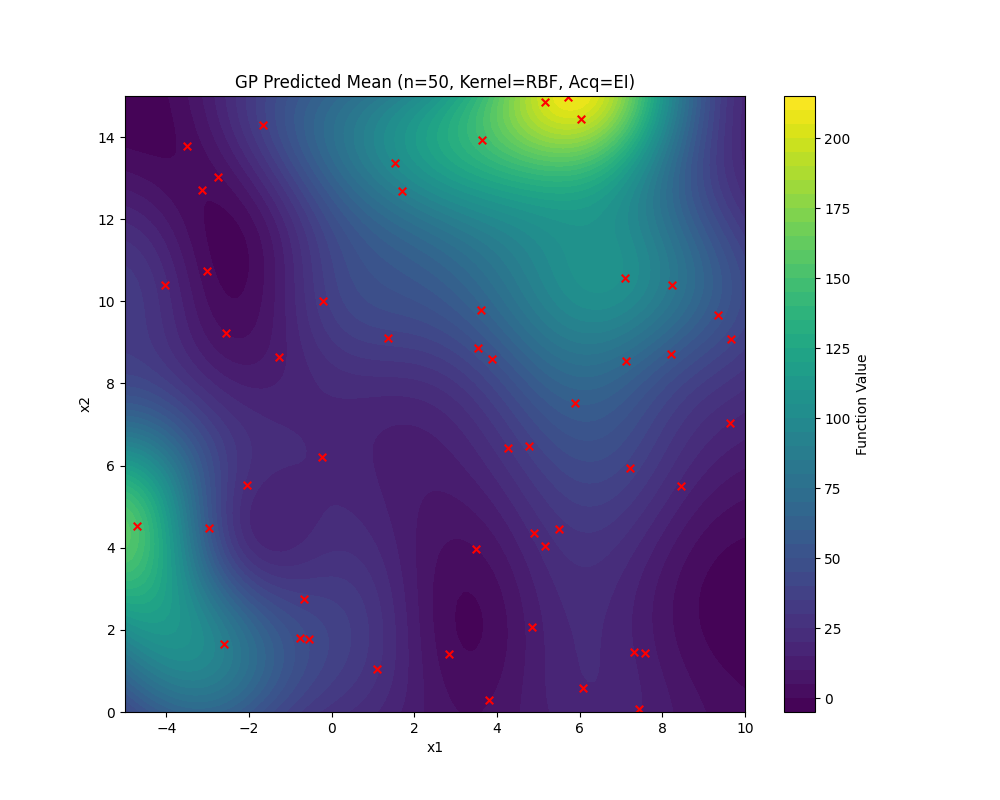
\includegraphics[width=0.225\textwidth]{../Task-02/plots/gp_mean_rbf_n50_EI.png} &
        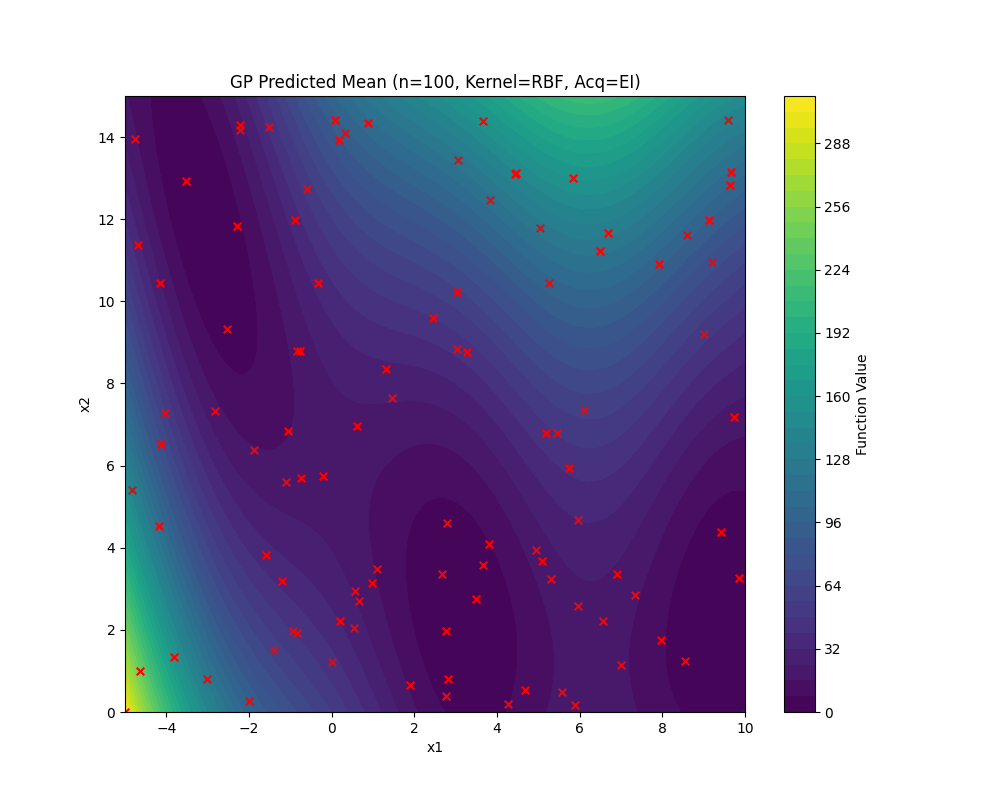
\includegraphics[width=0.225\textwidth]{../Task-02/plots/gp_mean_rbf_n100_EI.png} \\
        n=10 with EI & n=20 with EI & n=50 with EI & n=100 with EI \\[0.5em]
        
        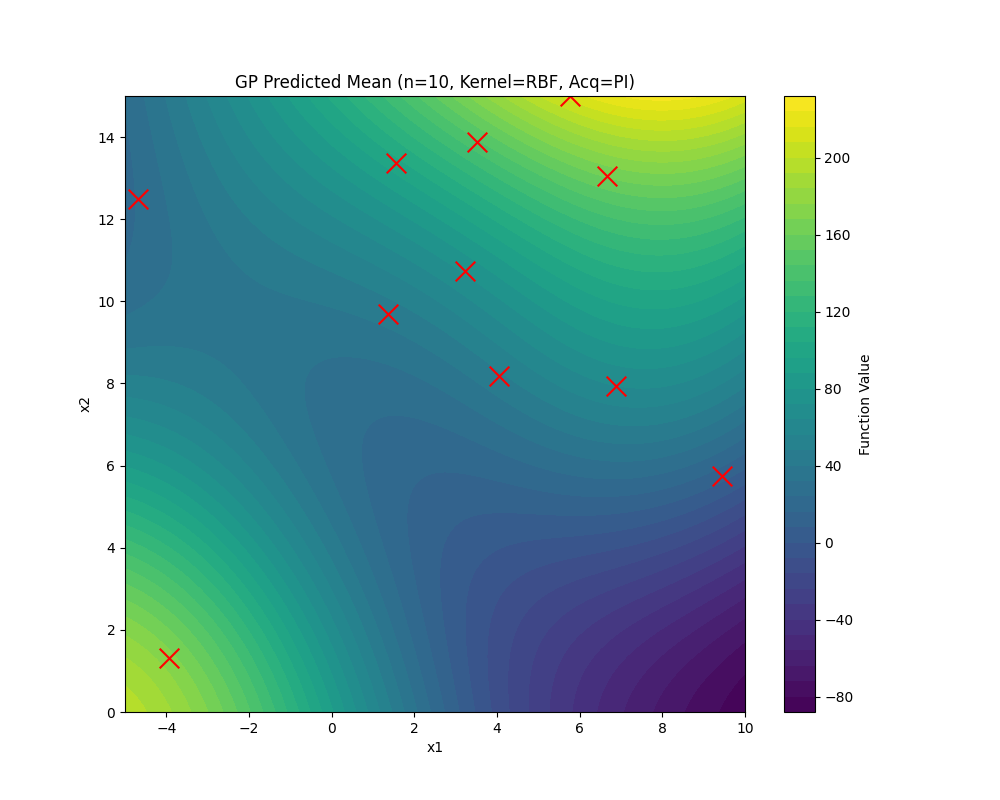
\includegraphics[width=0.225\textwidth]{../Task-02/plots/gp_mean_rbf_n10_PI.png} &
        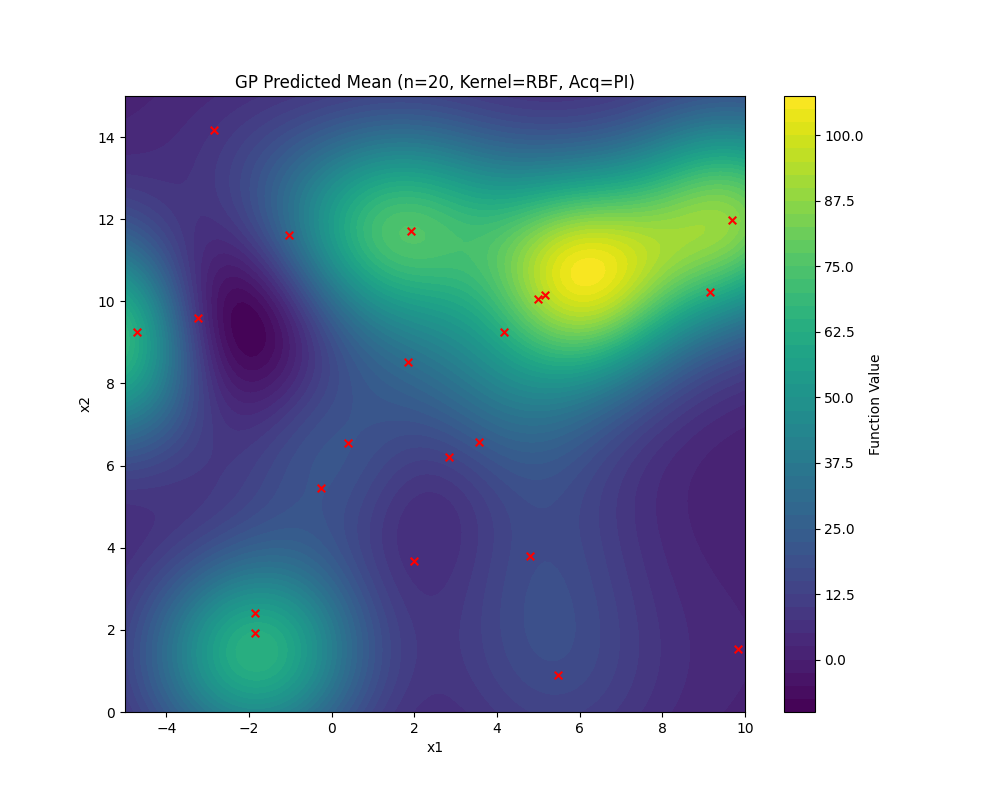
\includegraphics[width=0.225\textwidth]{../Task-02/plots/gp_mean_rbf_n20_PI.png} &
        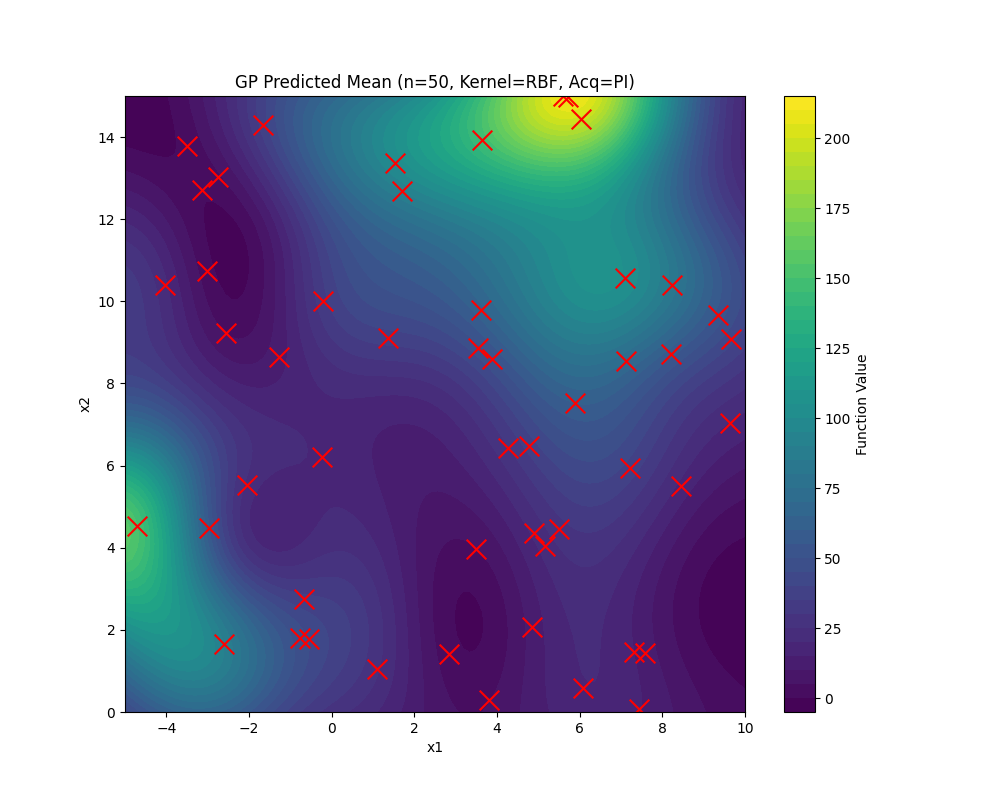
\includegraphics[width=0.225\textwidth]{../Task-02/plots/gp_mean_rbf_n50_PI.png} &
        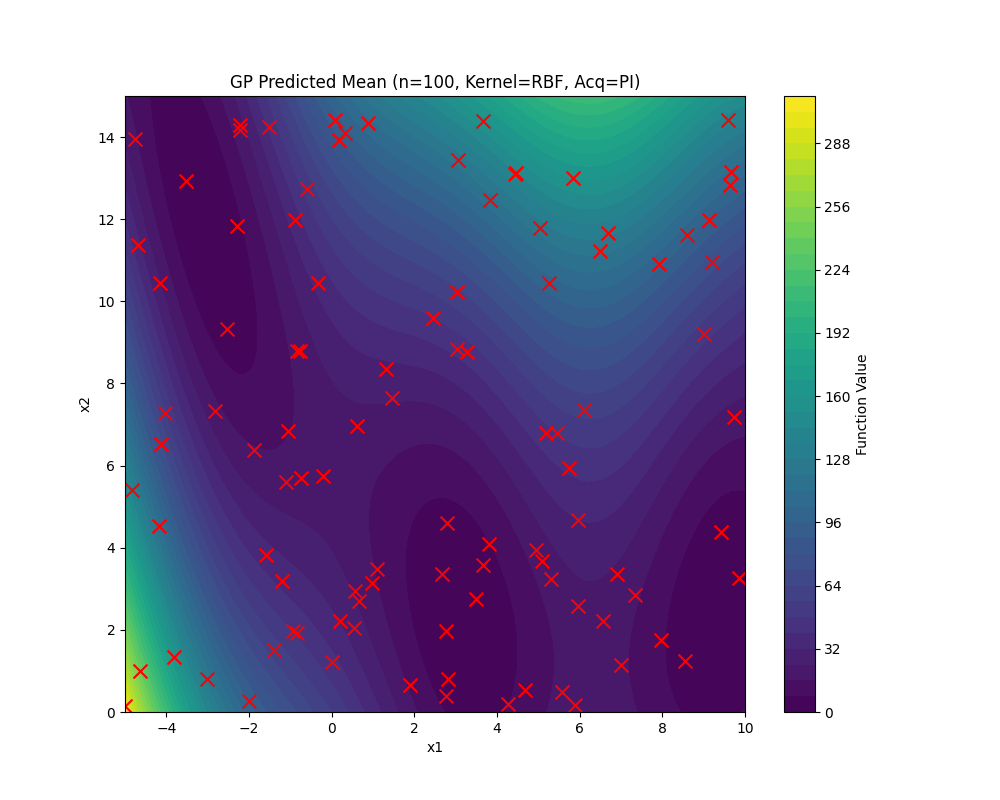
\includegraphics[width=0.225\textwidth]{../Task-02/plots/gp_mean_rbf_n100_PI.png} \\
        n=10 with PI & n=20 with PI & n=50 with PI & n=100 with PI \\
    \end{tabular}
    \caption{RBF kernel GP mean with different acquisition functions.}
    \label{fig:rbf_gp_mean}
\end{figure}

\begin{figure}[H]
    \centering
    \begin{tabular}{cccc}
        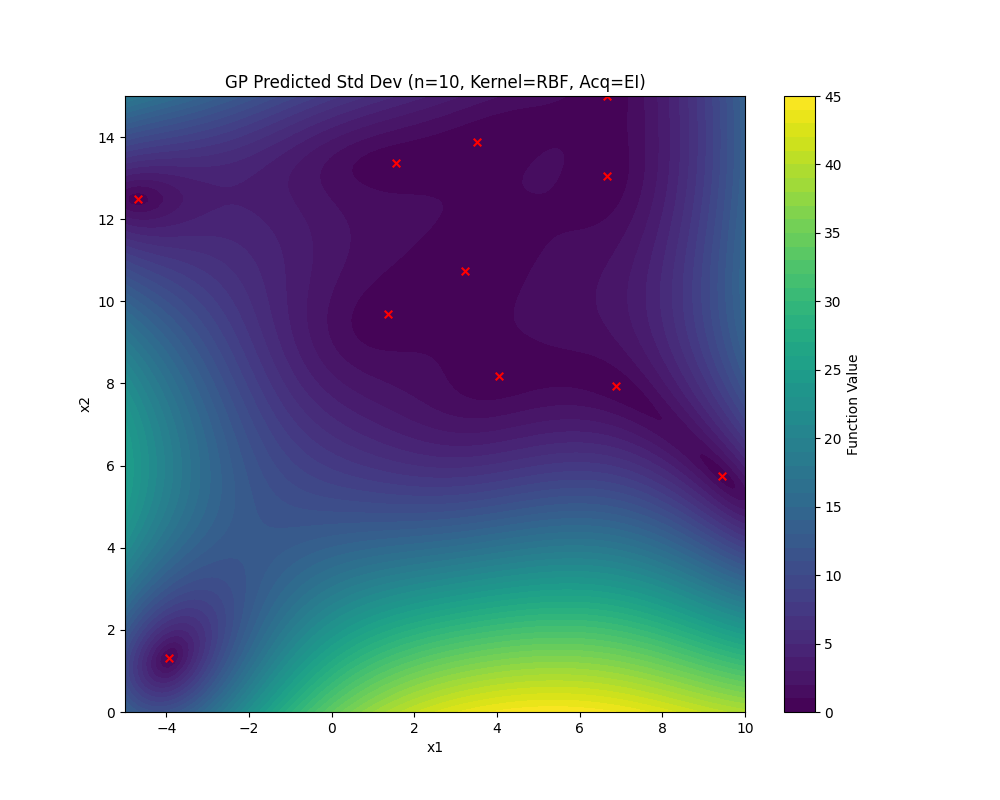
\includegraphics[width=0.225\textwidth]{../Task-02/plots/gp_std_rbf_n10_EI.png} &
        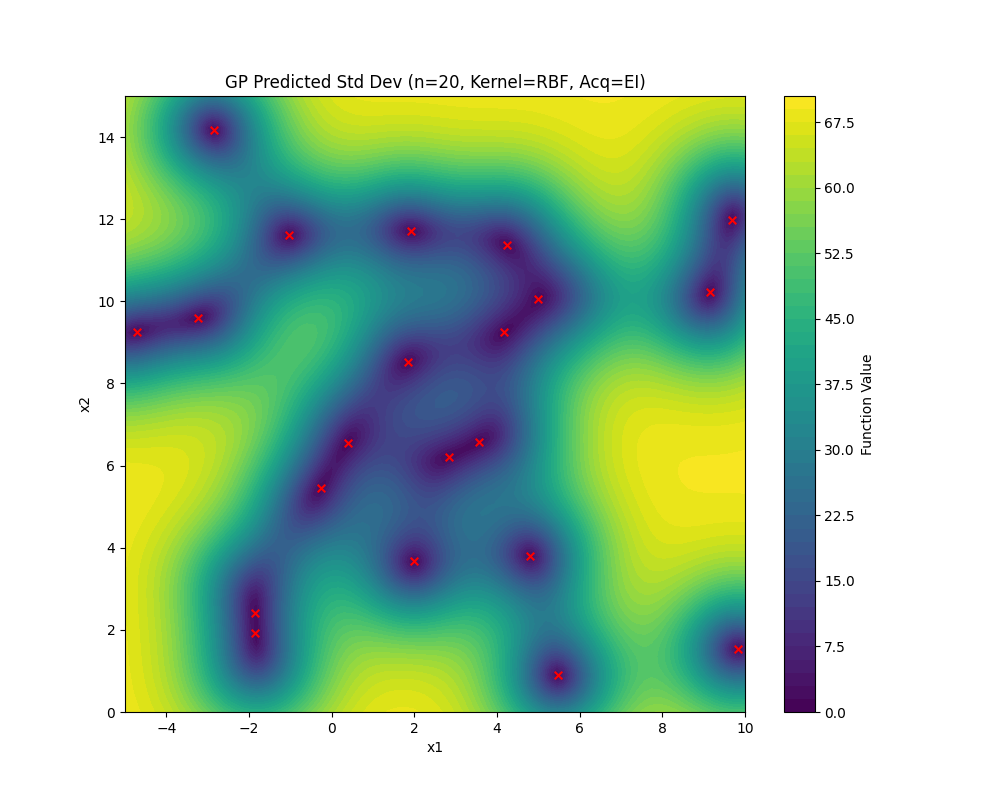
\includegraphics[width=0.225\textwidth]{../Task-02/plots/gp_std_rbf_n20_EI.png} &
        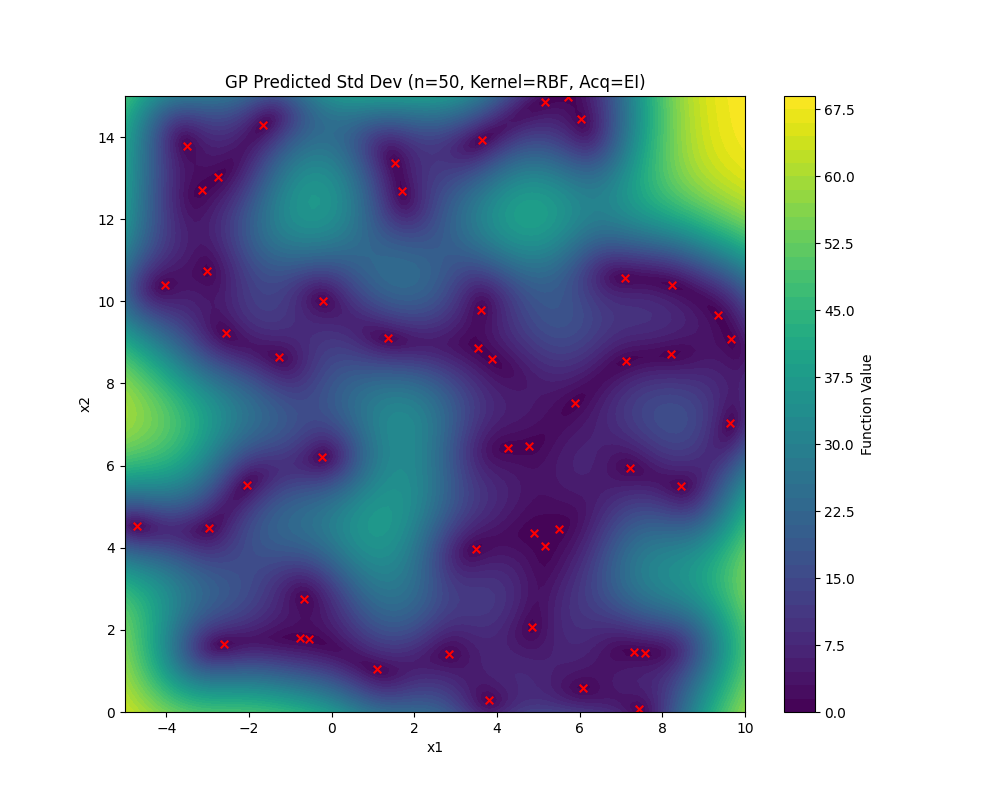
\includegraphics[width=0.225\textwidth]{../Task-02/plots/gp_std_rbf_n50_EI.png} &
        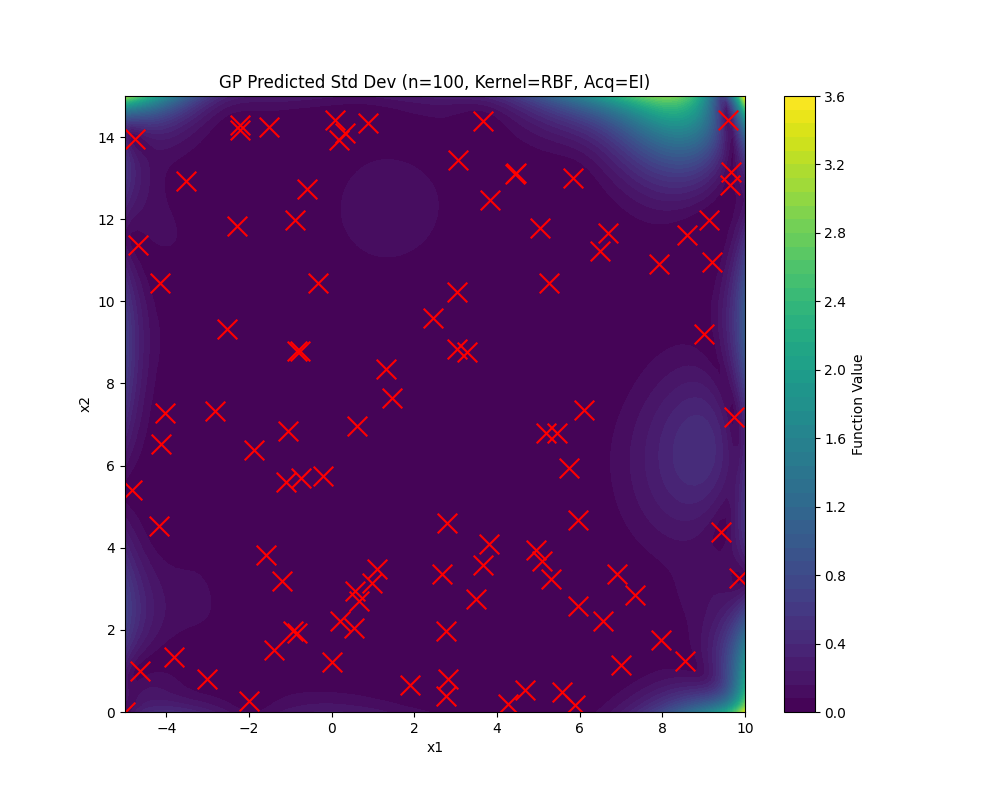
\includegraphics[width=0.225\textwidth]{../Task-02/plots/gp_std_rbf_n100_EI.png} \\
        n=10 with EI & n=20 with EI & n=50 with EI & n=100 with EI \\[0.5em]
        
        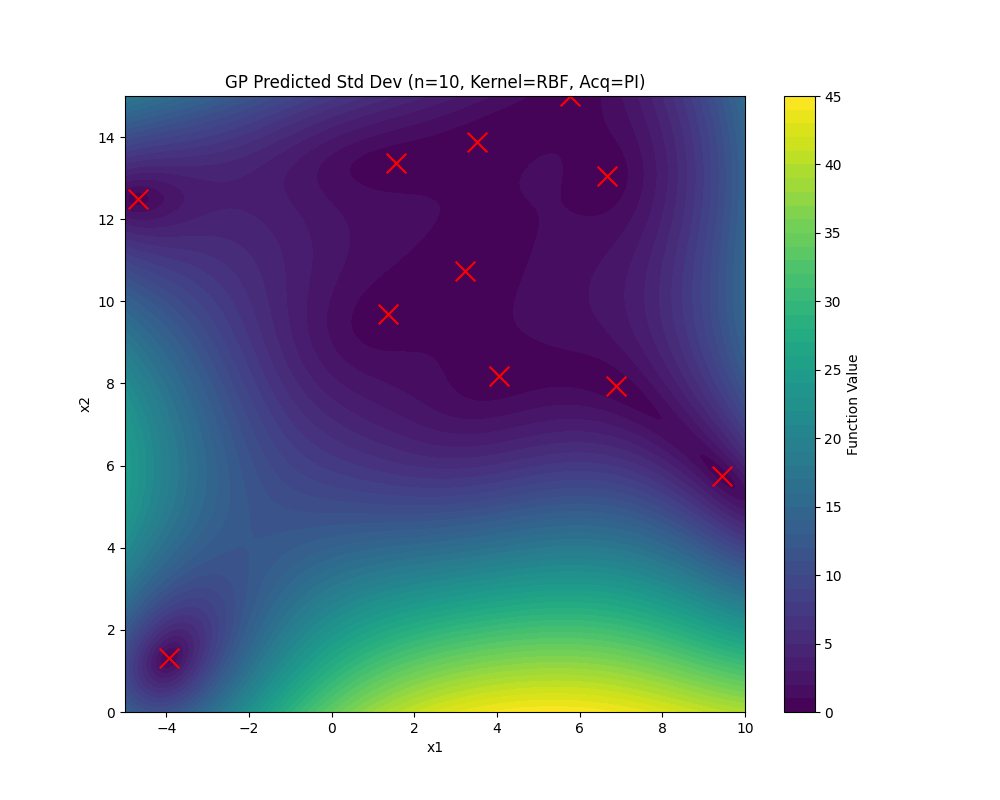
\includegraphics[width=0.225\textwidth]{../Task-02/plots/gp_std_rbf_n10_PI.png} &
        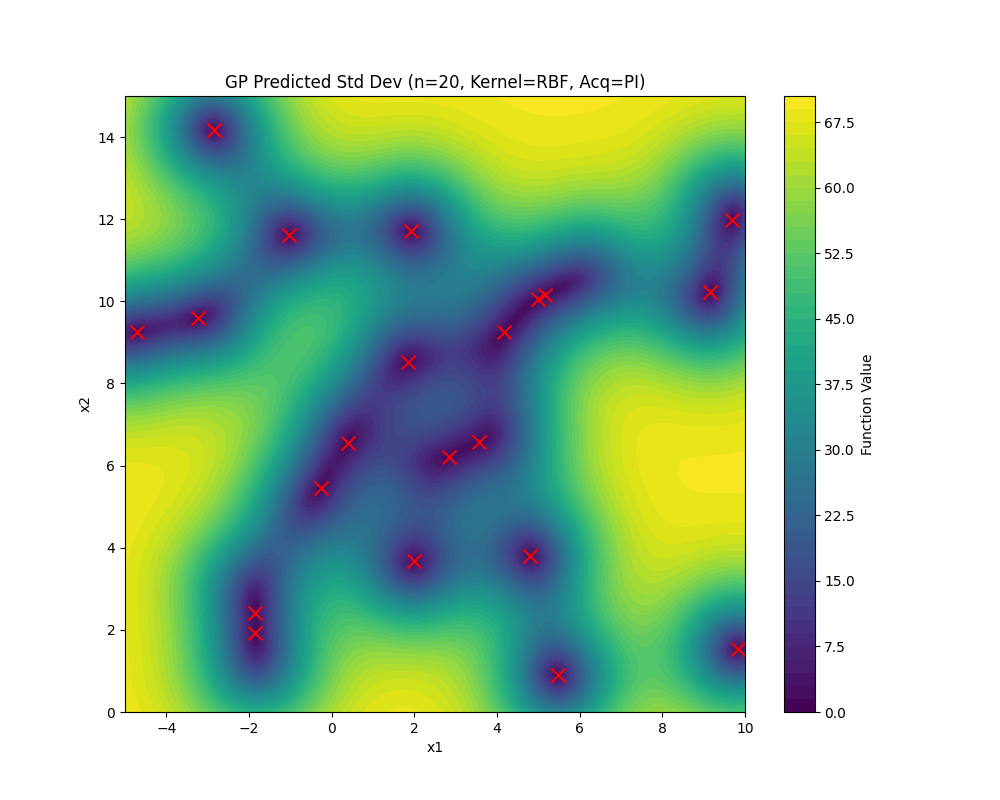
\includegraphics[width=0.225\textwidth]{../Task-02/plots/gp_std_rbf_n20_PI.png} &
        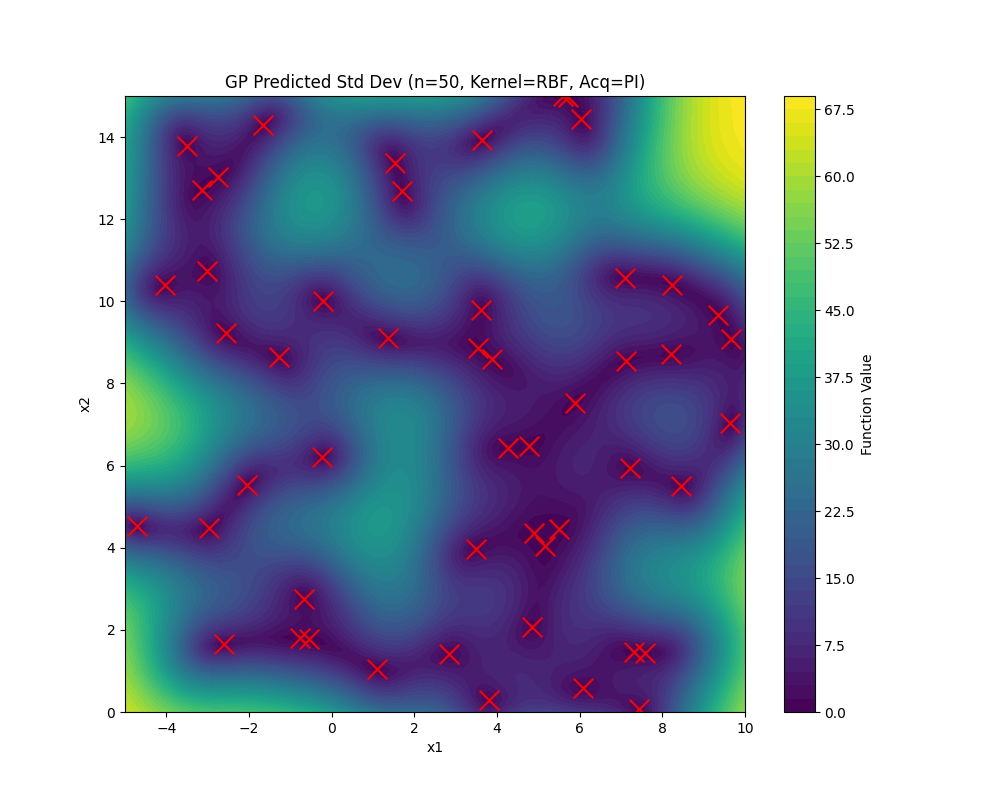
\includegraphics[width=0.225\textwidth]{../Task-02/plots/gp_std_rbf_n50_PI.png} &
        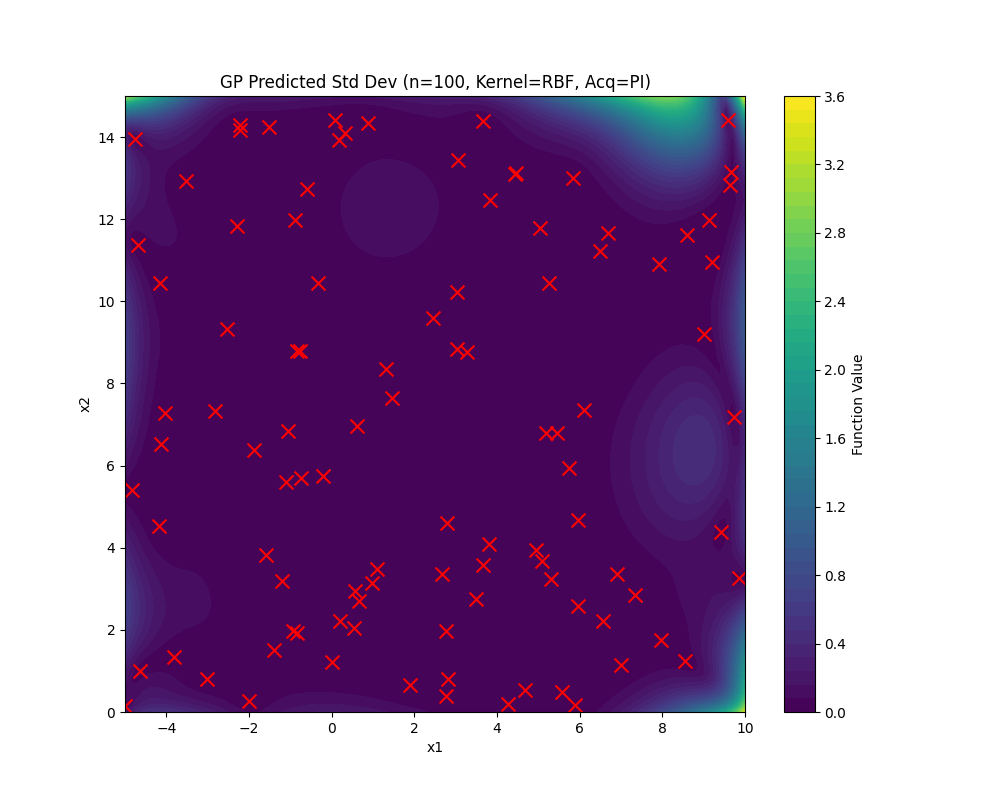
\includegraphics[width=0.225\textwidth]{../Task-02/plots/gp_std_rbf_n100_PI.png} \\
        n=10 with PI & n=20 with PI & n=50 with PI & n=100 with PI \\
    \end{tabular}
    \caption{RBF kernel GP standard deviation with different acquisition functions.}
    \label{fig:rbf_gp_std}
\end{figure}

\begin{figure}[H]
    \centering
    \begin{tabular}{cccc}
        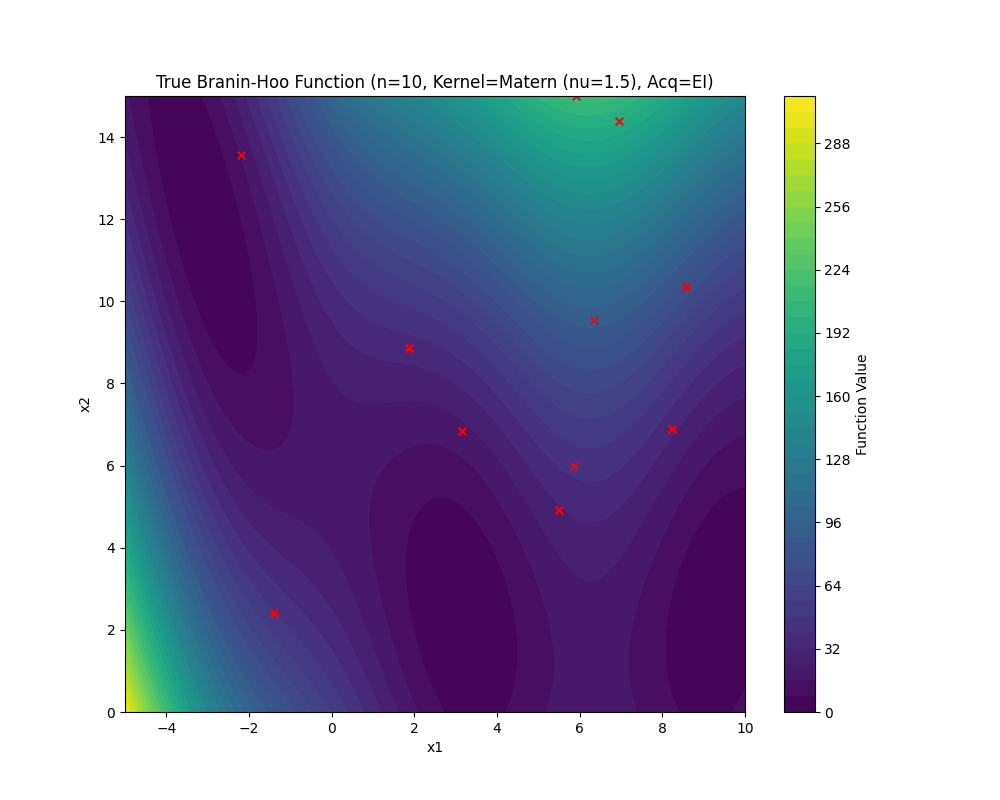
\includegraphics[width=0.225\textwidth]{../Task-02/plots/true_function_matern_n10_EI.png} &
        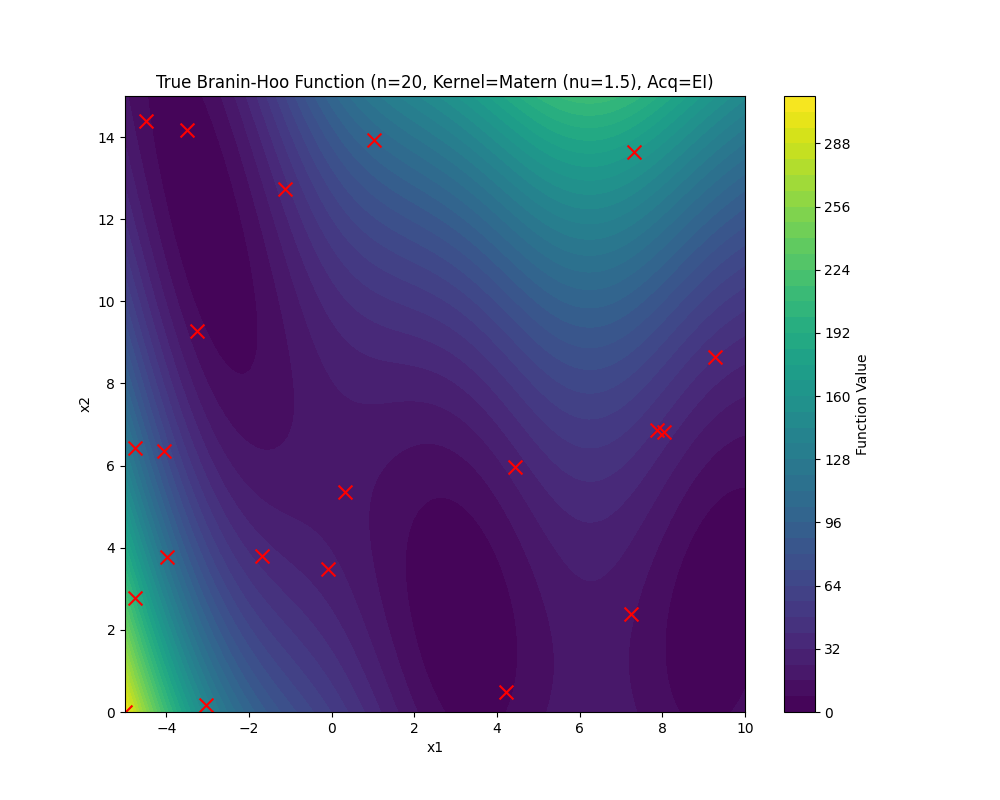
\includegraphics[width=0.225\textwidth]{../Task-02/plots/true_function_matern_n20_EI.png} &
        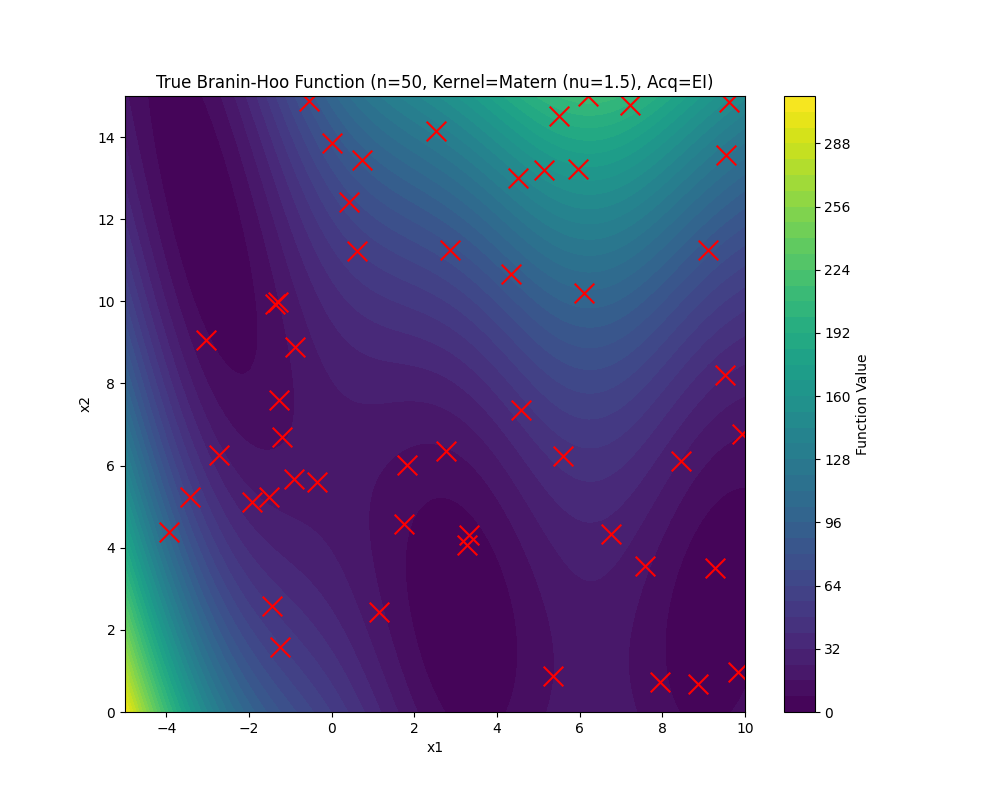
\includegraphics[width=0.225\textwidth]{../Task-02/plots/true_function_matern_n50_EI.png} &
        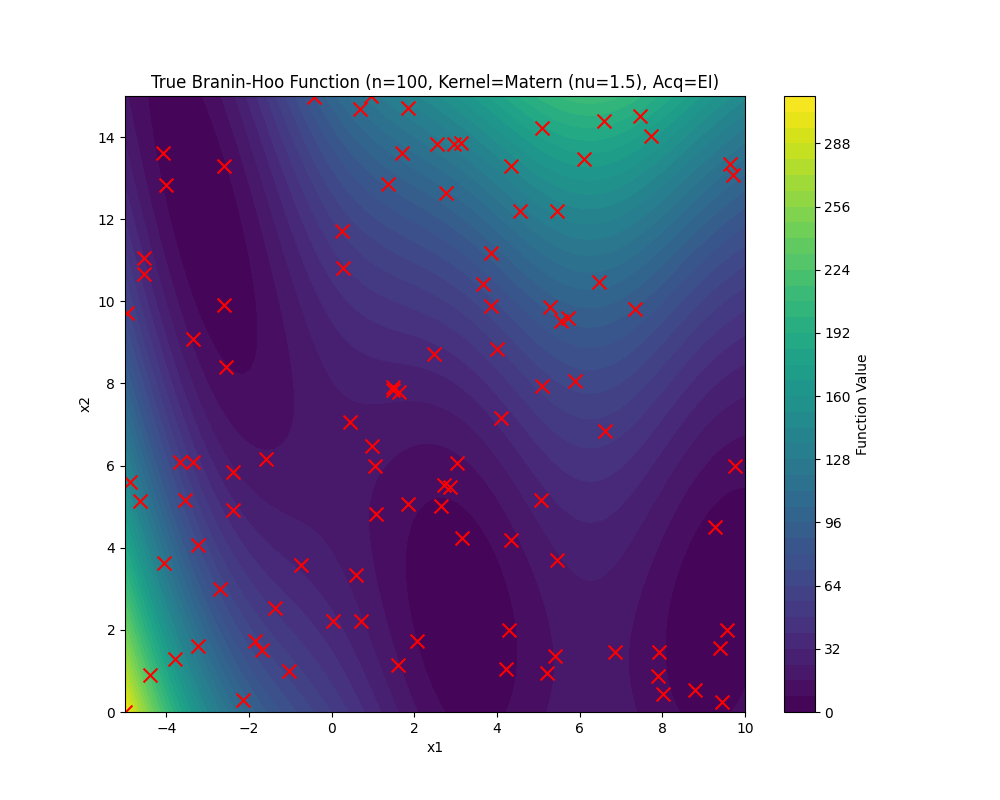
\includegraphics[width=0.225\textwidth]{../Task-02/plots/true_function_matern_n100_EI.png} \\
        n=10 with EI & n=20 with EI & n=50 with EI & n=100 with EI \\[0.5em]
        
        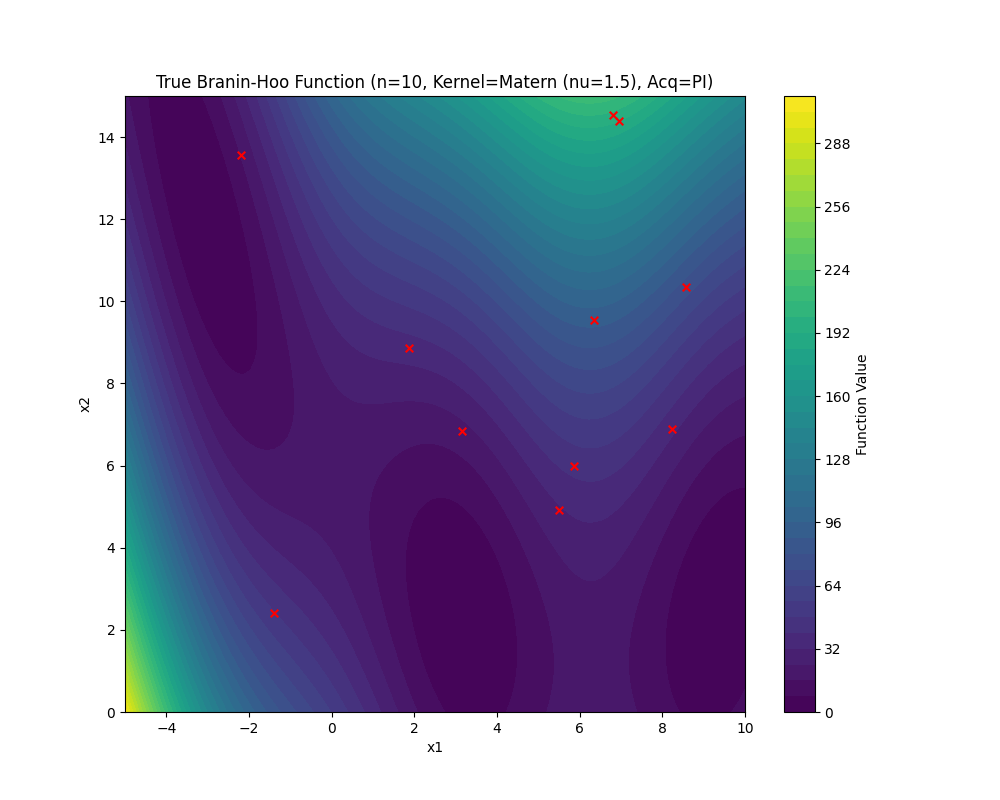
\includegraphics[width=0.225\textwidth]{../Task-02/plots/true_function_matern_n10_PI.png} &
        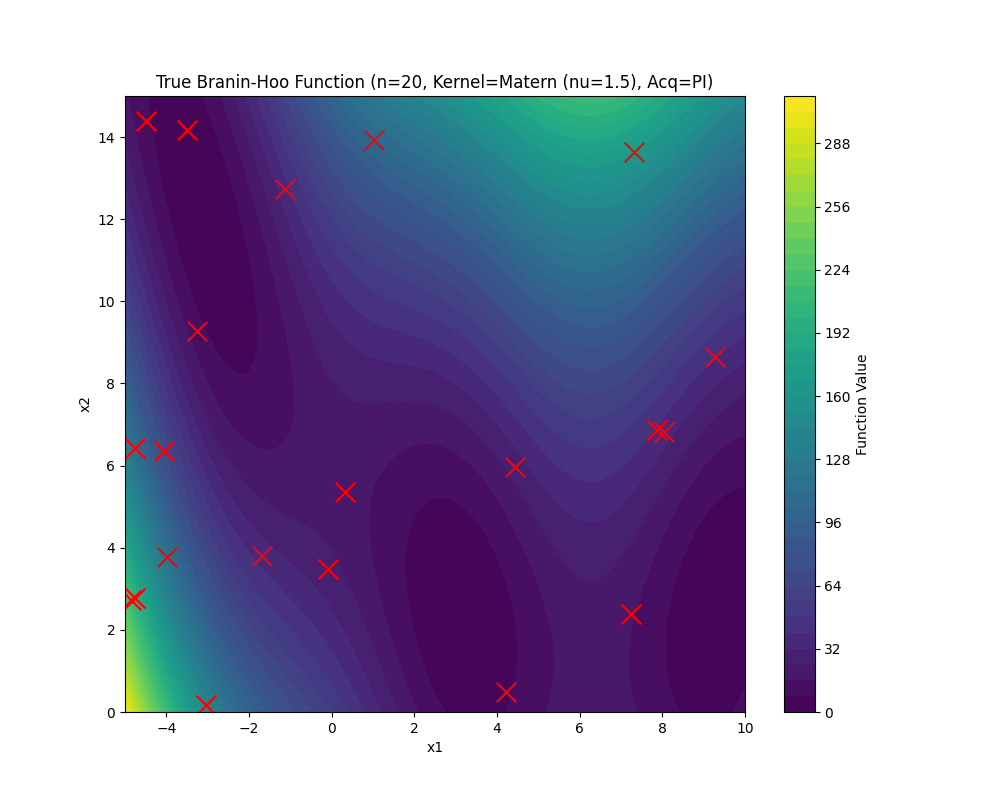
\includegraphics[width=0.225\textwidth]{../Task-02/plots/true_function_matern_n20_PI.png} &
        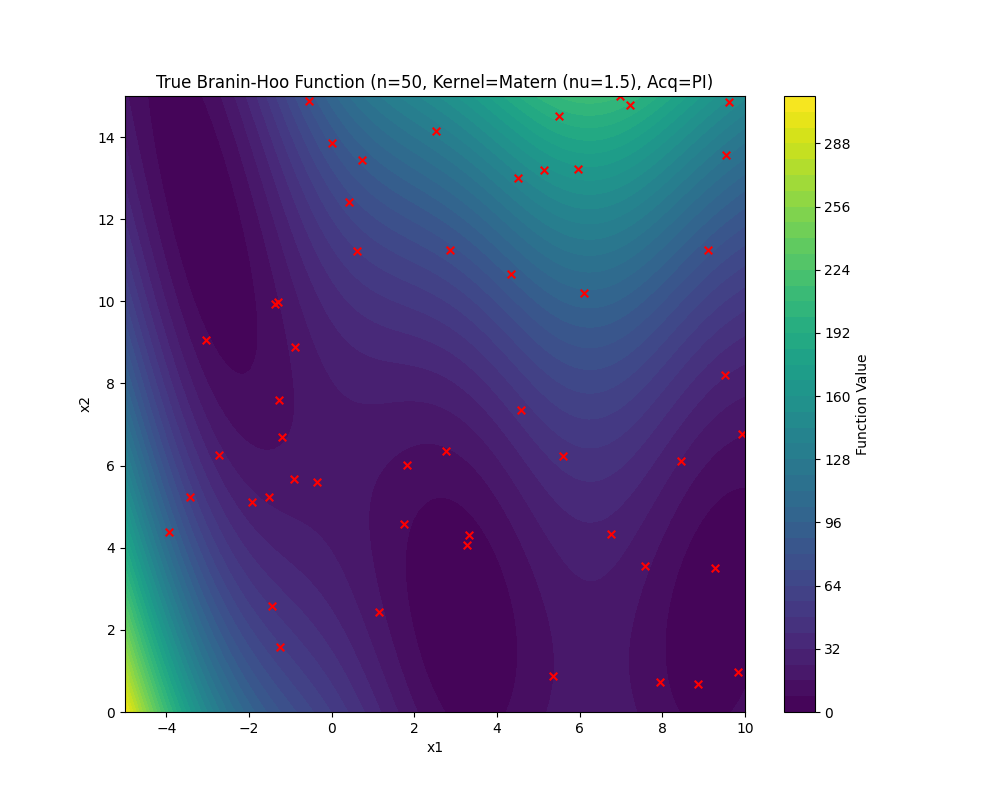
\includegraphics[width=0.225\textwidth]{../Task-02/plots/true_function_matern_n50_PI.png} &
        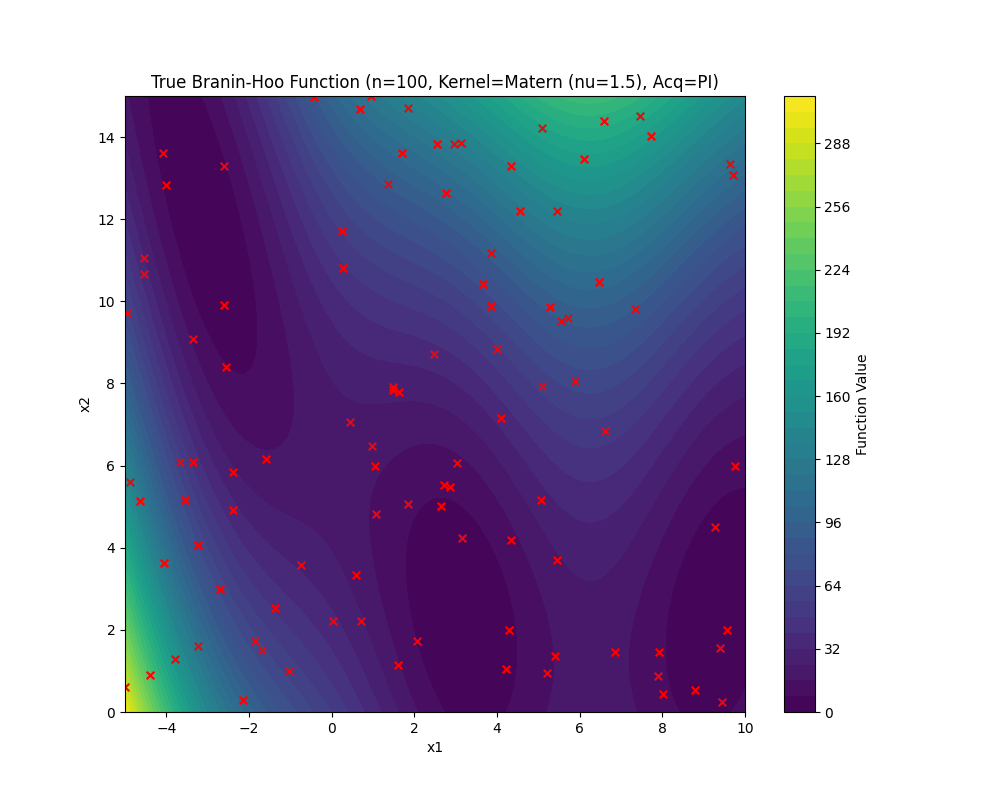
\includegraphics[width=0.225\textwidth]{../Task-02/plots/true_function_matern_n100_PI.png} \\
        n=10 with PI & n=20 with PI & n=50 with PI & n=100 with PI \\
    \end{tabular}
    \caption{Matern kernel true function with different acquisition functions.}
    \label{fig:matern_true_function}
\end{figure}

\begin{figure}[H]
    \centering
    \begin{tabular}{cccc}
        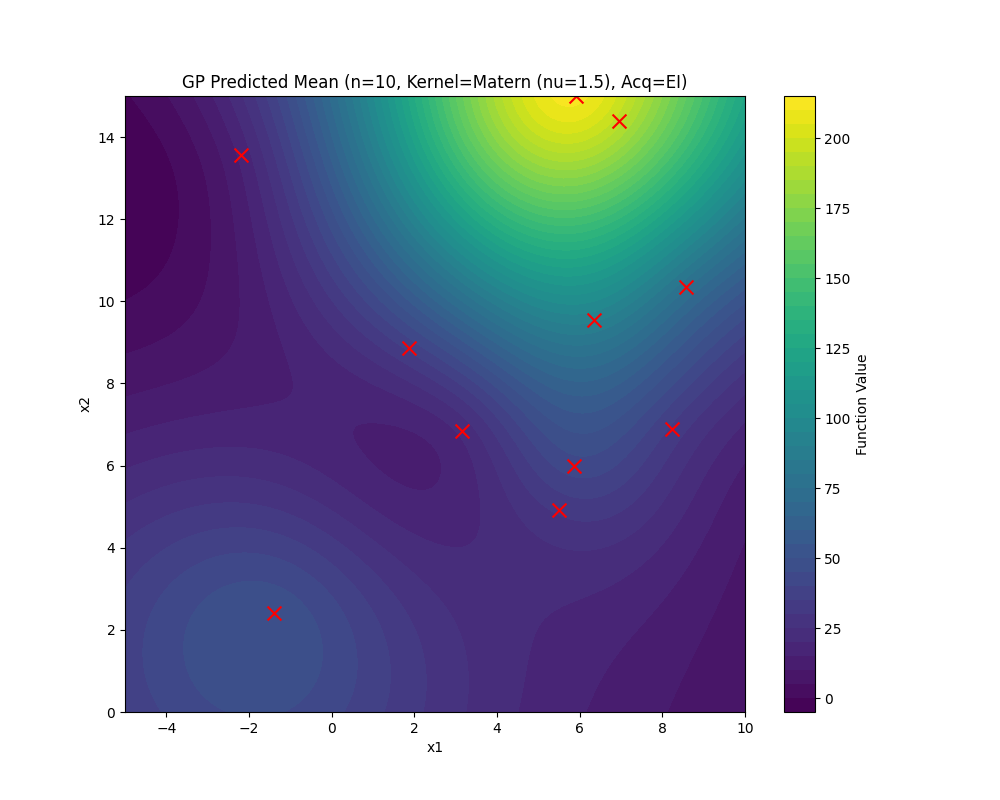
\includegraphics[width=0.225\textwidth]{../Task-02/plots/gp_mean_matern_n10_EI.png} &
        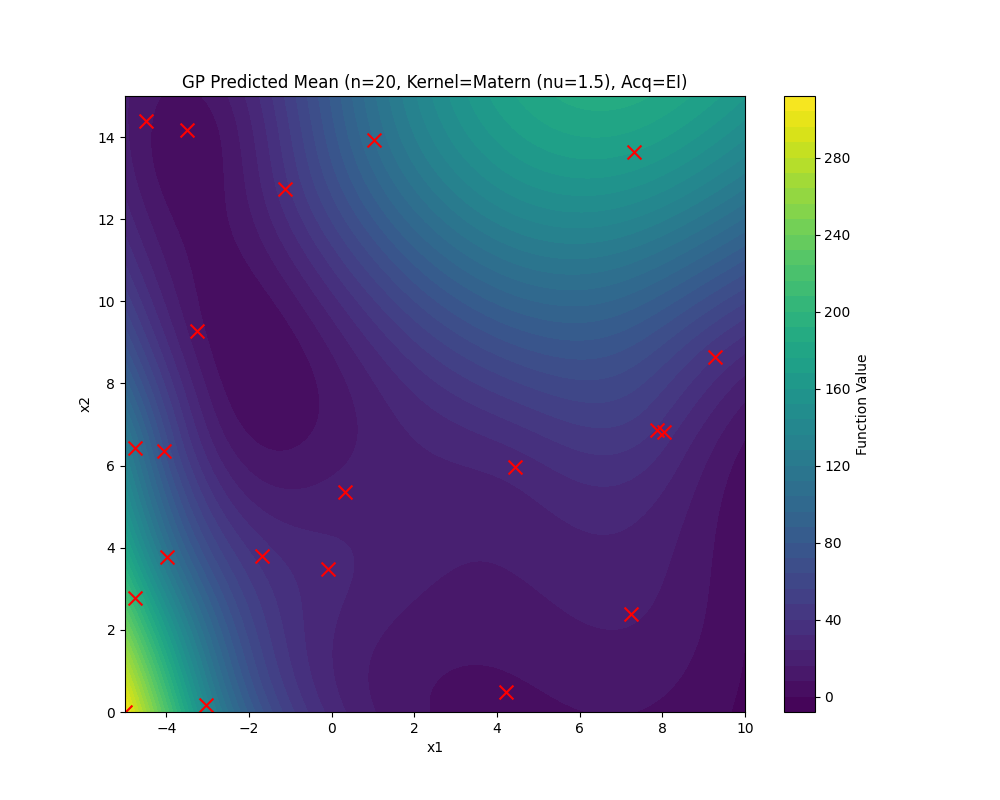
\includegraphics[width=0.225\textwidth]{../Task-02/plots/gp_mean_matern_n20_EI.png} &
        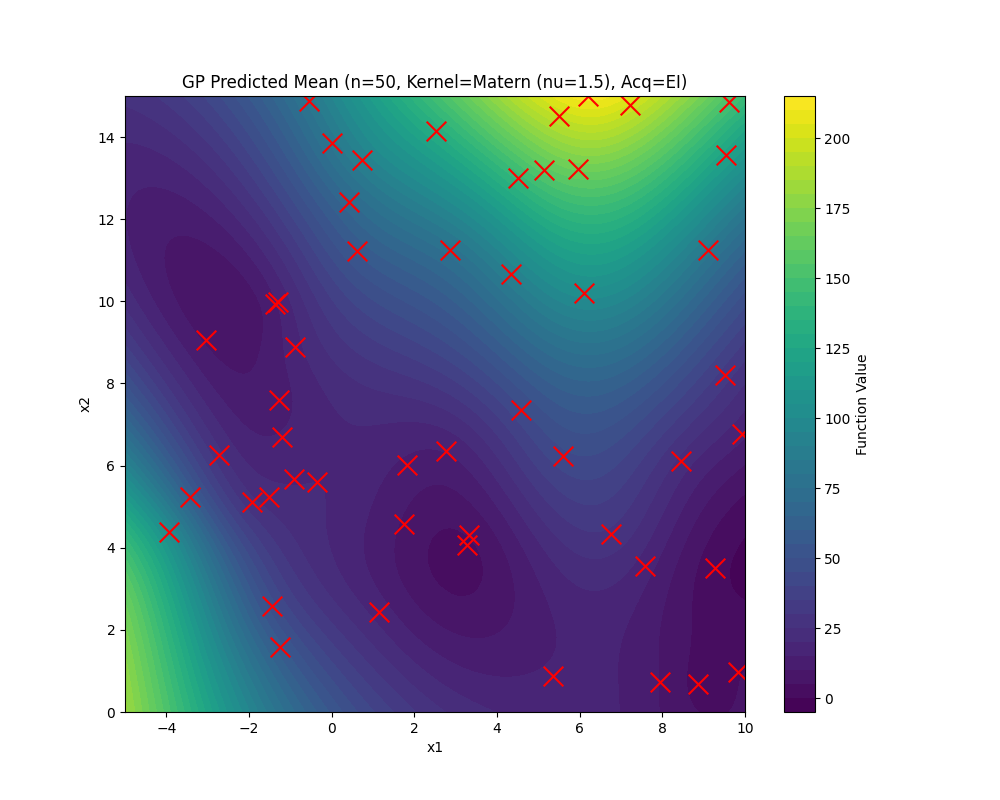
\includegraphics[width=0.225\textwidth]{../Task-02/plots/gp_mean_matern_n50_EI.png} &
        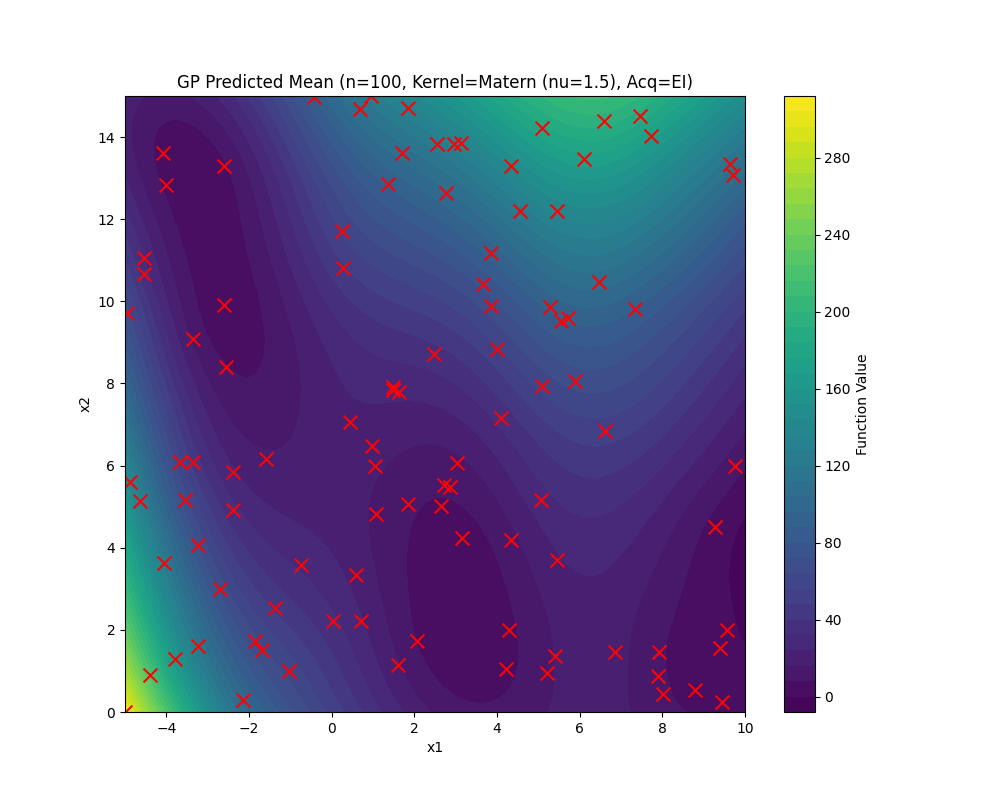
\includegraphics[width=0.225\textwidth]{../Task-02/plots/gp_mean_matern_n100_EI.png} \\
        n=10 with EI & n=20 with EI & n=50 with EI & n=100 with EI \\[0.5em]
        
        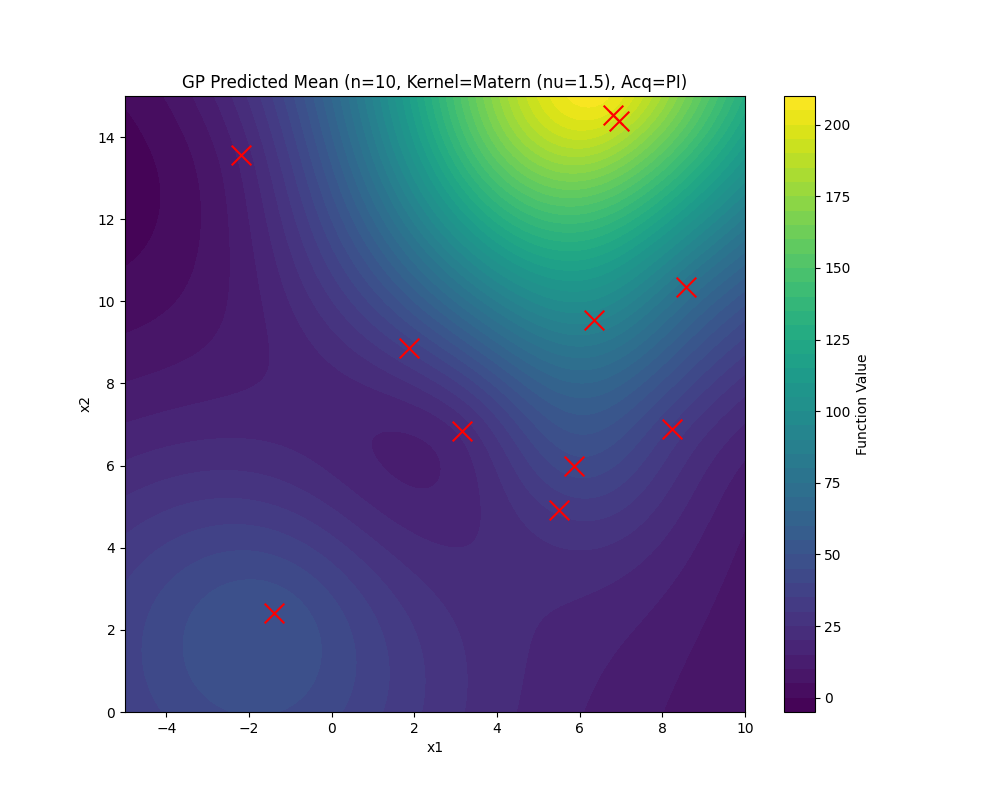
\includegraphics[width=0.225\textwidth]{../Task-02/plots/gp_mean_matern_n10_PI.png} &
        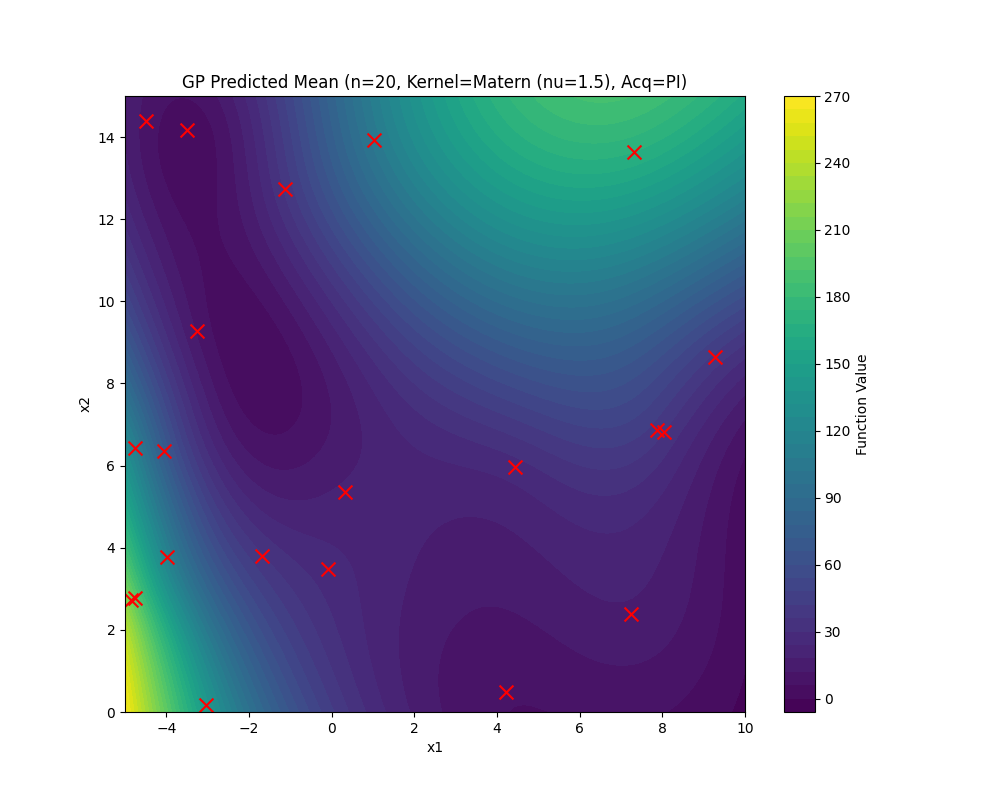
\includegraphics[width=0.225\textwidth]{../Task-02/plots/gp_mean_matern_n20_PI.png} &
        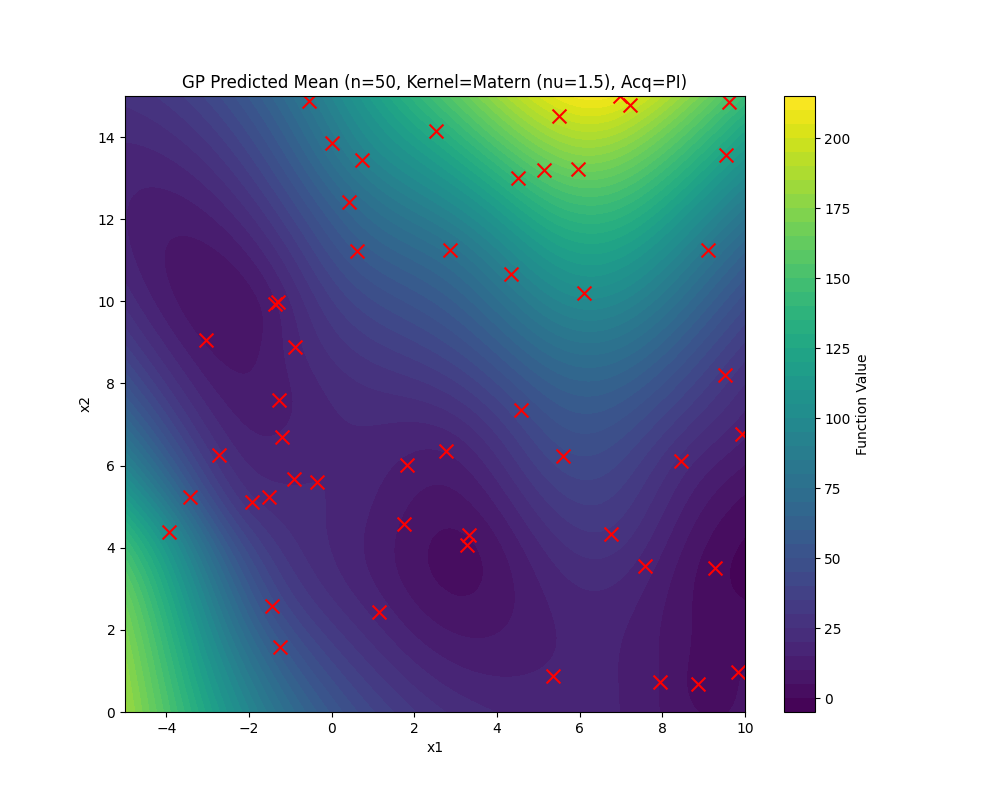
\includegraphics[width=0.225\textwidth]{../Task-02/plots/gp_mean_matern_n50_PI.png} &
        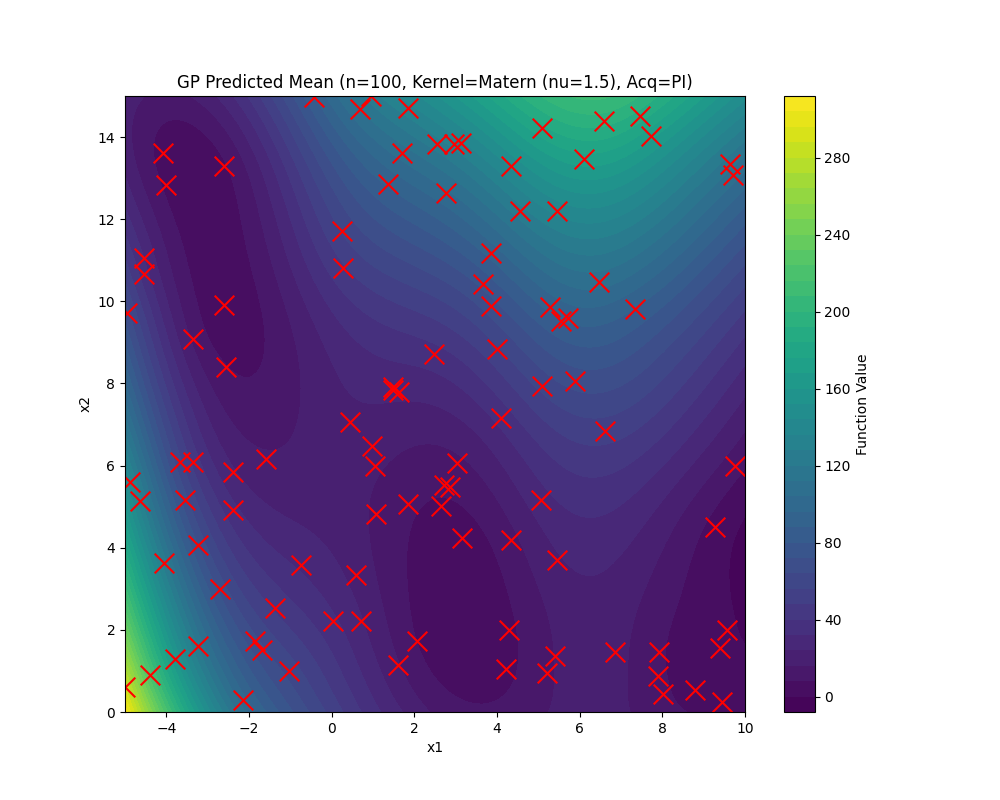
\includegraphics[width=0.225\textwidth]{../Task-02/plots/gp_mean_matern_n100_PI.png} \\
        n=10 with PI & n=20 with PI & n=50 with PI & n=100 with PI \\
    \end{tabular}
    \caption{Matern kernel GP mean with different acquisition functions.}
    \label{fig:matern_gp_mean}
\end{figure}

\begin{figure}[H]
    \centering
    \begin{tabular}{cccc}
        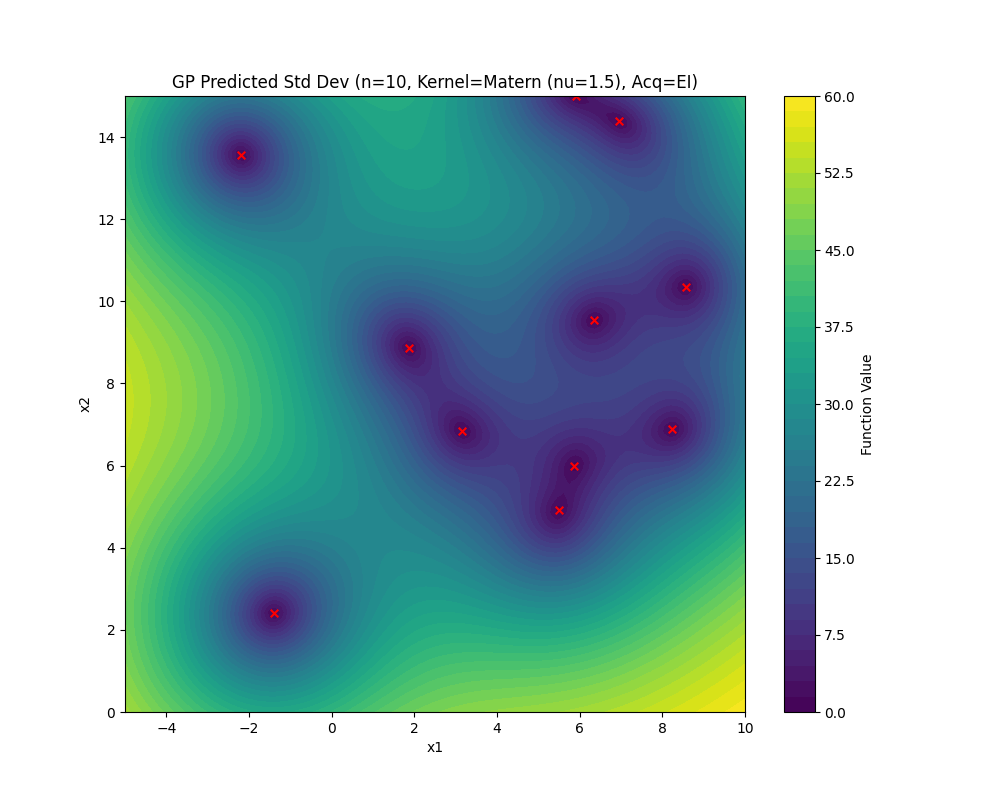
\includegraphics[width=0.225\textwidth]{../Task-02/plots/gp_std_matern_n10_EI.png} &
        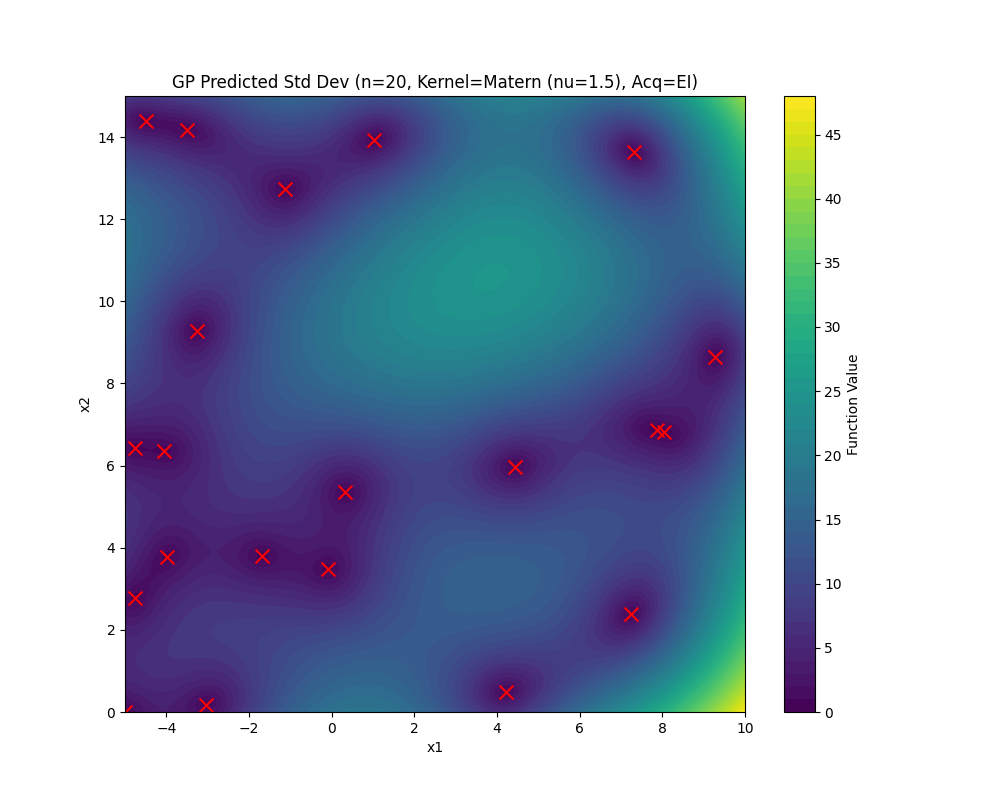
\includegraphics[width=0.225\textwidth]{../Task-02/plots/gp_std_matern_n20_EI.png} &
        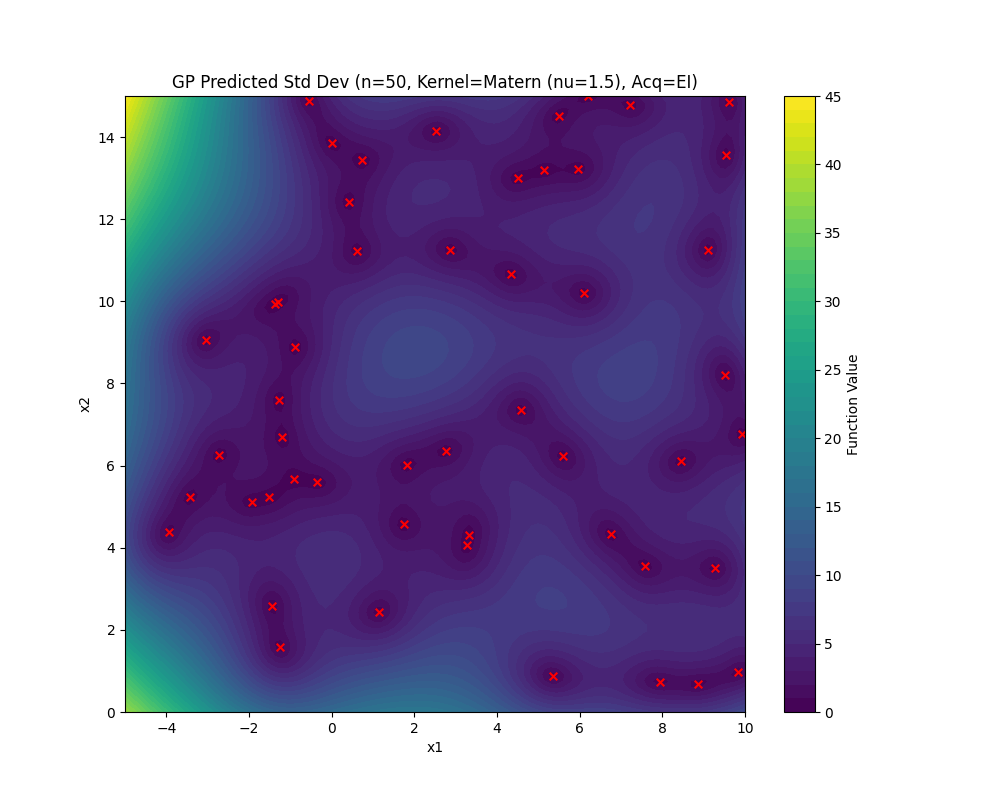
\includegraphics[width=0.225\textwidth]{../Task-02/plots/gp_std_matern_n50_EI.png} &
        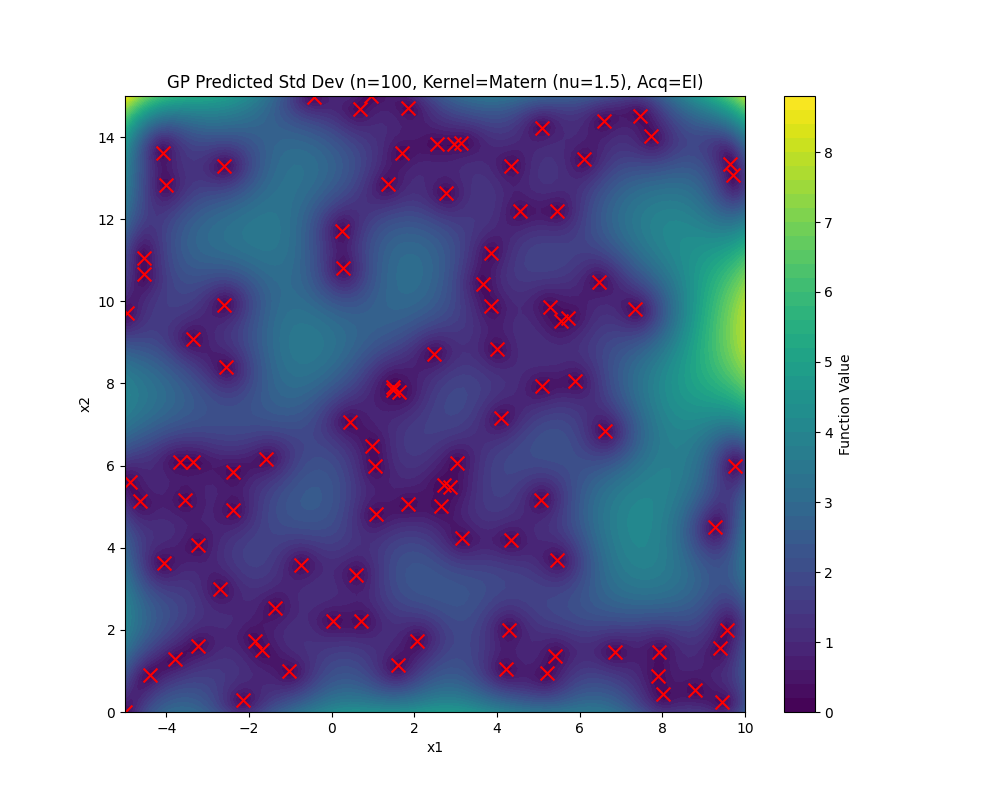
\includegraphics[width=0.225\textwidth]{../Task-02/plots/gp_std_matern_n100_EI.png} \\
        n=10 with EI & n=20 with EI & n=50 with EI & n=100 with EI \\[0.5em]
        
        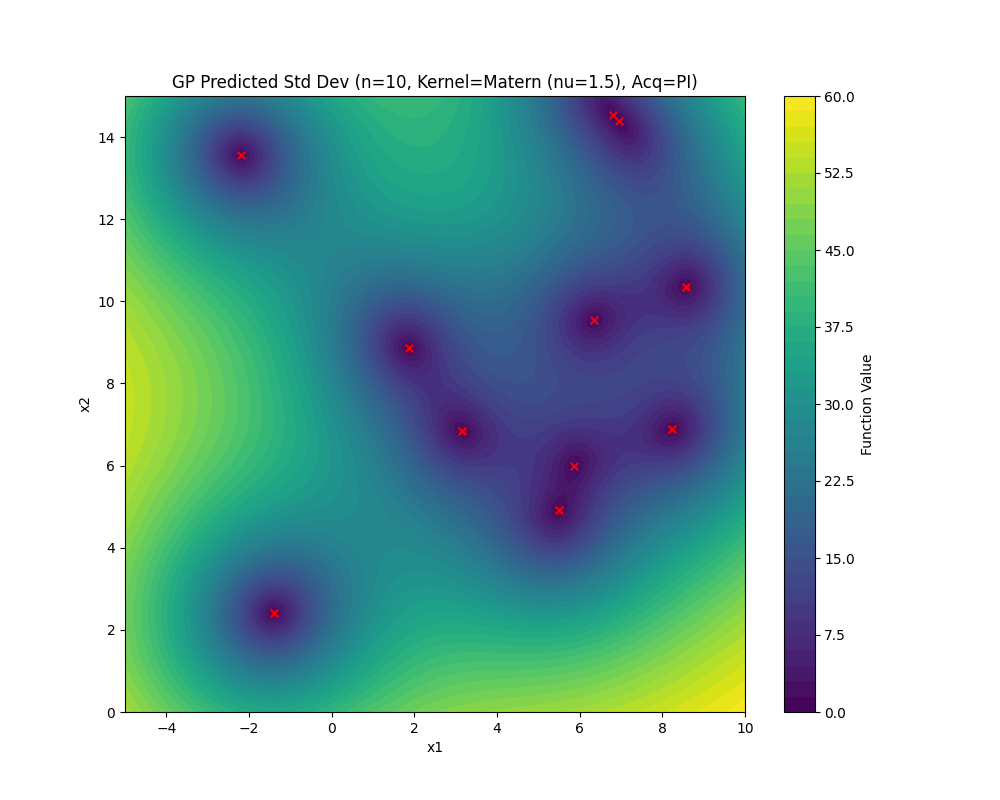
\includegraphics[width=0.225\textwidth]{../Task-02/plots/gp_std_matern_n10_PI.png} &
        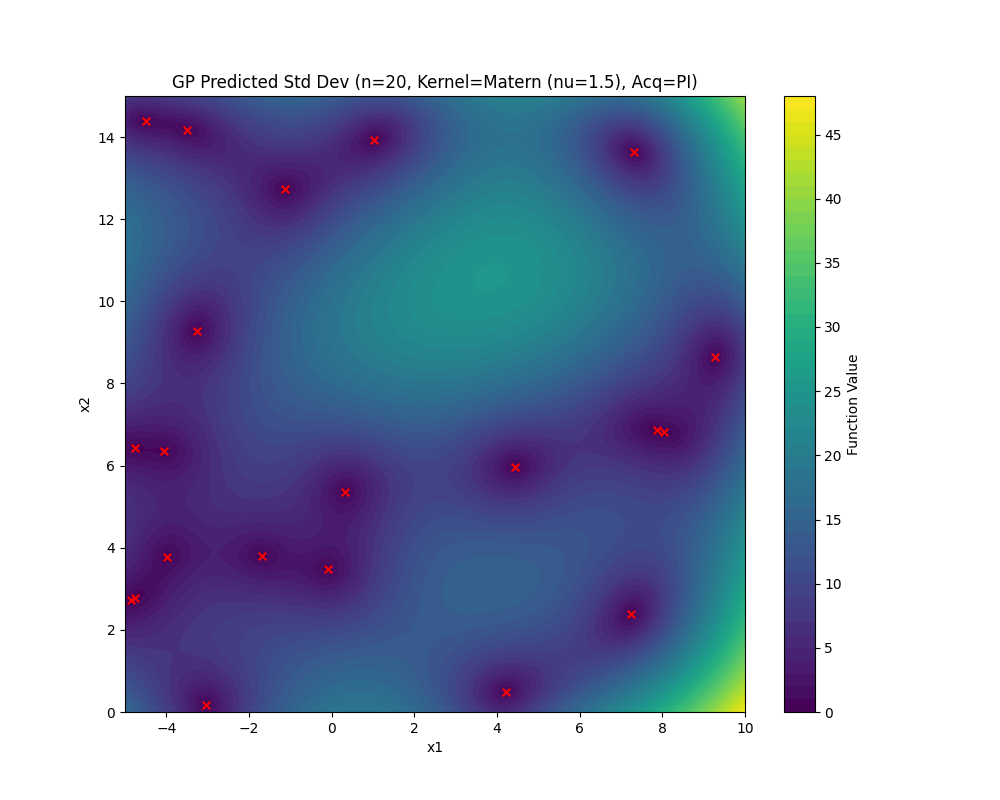
\includegraphics[width=0.225\textwidth]{../Task-02/plots/gp_std_matern_n20_PI.png} &
        \includegraphics[width=0.225\textwidth]{../Task-02/plots/gp_std_matern_n50_PI.png} &
        \includegraphics[width=0.225\textwidth]{../Task-02/plots/gp_std_matern_n100_PI.png} \\
        n=10 with PI & n=20 with PI & n=50 with PI & n=100 with PI \\
    \end{tabular}
    \caption{Matern kernel GP standard deviation with different acquisition functions.}
    \label{fig:matern_gp_std}
\end{figure}

\begin{figure}[H]
    \centering
    \begin{tabular}{cccc}
        \includegraphics[width=0.225\textwidth]{../Task-02/plots/true_function_rational_quadratic_n10_EI.png} &
        \includegraphics[width=0.225\textwidth]{../Task-02/plots/true_function_rational_quadratic_n20_EI.png} &
        \includegraphics[width=0.225\textwidth]{../Task-02/plots/true_function_rational_quadratic_n50_EI.png} &
        \includegraphics[width=0.225\textwidth]{../Task-02/plots/true_function_rational_quadratic_n100_EI.png} \\
        n=10 with EI & n=20 with EI & n=50 with EI & n=100 with EI \\[0.5em]
        
        \includegraphics[width=0.225\textwidth]{../Task-02/plots/true_function_rational_quadratic_n10_PI.png} &
        \includegraphics[width=0.225\textwidth]{../Task-02/plots/true_function_rational_quadratic_n20_PI.png} &
        \includegraphics[width=0.225\textwidth]{../Task-02/plots/true_function_rational_quadratic_n50_PI.png} &
        \includegraphics[width=0.225\textwidth]{../Task-02/plots/true_function_rational_quadratic_n100_PI.png} \\
        n=10 with PI & n=20 with PI & n=50 with PI & n=100 with PI \\
    \end{tabular}
    \caption{Rational Quadratic kernel true function with different acquisition functions.}
    \label{fig:rational_quadratic_true_function}
\end{figure}

\begin{figure}[H]
    \centering
    \begin{tabular}{cccc}
        \includegraphics[width=0.225\textwidth]{../Task-02/plots/gp_mean_rational_quadratic_n10_EI.png} &
        \includegraphics[width=0.225\textwidth]{../Task-02/plots/gp_mean_rational_quadratic_n20_EI.png} &
        \includegraphics[width=0.225\textwidth]{../Task-02/plots/gp_mean_rational_quadratic_n50_EI.png} &
        \includegraphics[width=0.225\textwidth]{../Task-02/plots/gp_mean_rational_quadratic_n100_EI.png} \\
        n=10 with EI & n=20 with EI & n=50 with EI & n=100 with EI \\[0.5em]
        
        \includegraphics[width=0.225\textwidth]{../Task-02/plots/gp_mean_rational_quadratic_n10_PI.png} &
        \includegraphics[width=0.225\textwidth]{../Task-02/plots/gp_mean_rational_quadratic_n20_PI.png} &
        \includegraphics[width=0.225\textwidth]{../Task-02/plots/gp_mean_rational_quadratic_n50_PI.png} &
        \includegraphics[width=0.225\textwidth]{../Task-02/plots/gp_mean_rational_quadratic_n100_PI.png} \\
        n=10 with PI & n=20 with PI & n=50 with PI & n=100 with PI \\
    \end{tabular}
    \caption{Rational Quadratic kernel GP mean with different acquisition functions.}
    \label{fig:rational_quadratic_gp_mean}
\end{figure}

\begin{figure}[H]
    \centering
    \begin{tabular}{cccc}
        \includegraphics[width=0.225\textwidth]{../Task-02/plots/gp_std_rational_quadratic_n10_EI.png} &
        \includegraphics[width=0.225\textwidth]{../Task-02/plots/gp_std_rational_quadratic_n20_EI.png} &
        \includegraphics[width=0.225\textwidth]{../Task-02/plots/gp_std_rational_quadratic_n50_EI.png} &
        \includegraphics[width=0.225\textwidth]{../Task-02/plots/gp_std_rational_quadratic_n100_EI.png} \\
        n=10 with EI & n=20 with EI & n=50 with EI & n=100 with EI \\[0.5em]
        
        \includegraphics[width=0.225\textwidth]{../Task-02/plots/gp_std_rational_quadratic_n10_PI.png} &
        \includegraphics[width=0.225\textwidth]{../Task-02/plots/gp_std_rational_quadratic_n20_PI.png} &
        \includegraphics[width=0.225\textwidth]{../Task-02/plots/gp_std_rational_quadratic_n50_PI.png} &
        \includegraphics[width=0.225\textwidth]{../Task-02/plots/gp_std_rational_quadratic_n100_PI.png} \\
        n=10 with PI & n=20 with PI & n=50 with PI & n=100 with PI \\
    \end{tabular}
    \caption{Rational Quadratic kernel GP standard deviation with different acquisition functions.}
    \label{fig:rational_quadratic_gp_std}
\end{figure}

\subsection*{Observations}

\begin{enumerate}
    \item \textbf{Effect of Sample Size ($n$):}
    \begin{itemize}
        \item As $n$ increases, the GP mean becomes more accurate and closely resembles the true function.
        \item The standard deviation decreases, indicating improved confidence in predictions.
    \end{itemize}

    \item \textbf{EI vs. PI:}
    \begin{itemize}
        \item \textbf{EI} promotes better exploration, especially at smaller $n$, by sampling more diverse regions.
        \item \textbf{PI} is more exploitative and often clusters samples, potentially leading to suboptimal local solutions.
    \end{itemize}

    \item \textbf{Kernel Behavior:}
    \begin{itemize}
        \item \textbf{RBF Kernel:} Produces smooth, globally consistent approximations. Performs well across all $n$.
        \item \textbf{Matern Kernel:} Shows more localized variations; slower to converge but captures fine-grained features.
        \item \textbf{Rational Quadratic Kernel:} Balances smoothness and local adaptability. Strong performance even at low $n$.
    \end{itemize}

    \item \textbf{Uncertainty Patterns:}
    \begin{itemize}
        \item Higher uncertainty (GP std dev) is seen at the edges or unsampled regions.
        \item These areas shrink as $n$ increases, particularly with EI-based acquisition.
    \end{itemize}
\end{enumerate}

\section*{Contributions}

\begin{itemize}
    \item \textbf{Deeptanshu Malu}:
    \begin{enumerate}
        \item Formulated the trie data structure design for Task 1.
        \item Coded the multi head decoding algorithm for Task 2.
    \end{enumerate}

    \item \textbf{Deevyanshu Malu}:
    \begin{enumerate}
        \item Coded the trie data structure and the constrained decoding algorithm for Task 1.
        \item Coded the multi head decoding algorithm for Task 2.
    \end{enumerate}

    \item \textbf{Neel Rambhia}:
    \begin{enumerate}
        \item Completed all decoding algorithms in Task 0.
        \item Coded the single head decoding algorithm for Task 2.
    \end{enumerate}
\end{itemize}

\section*{Acknowledgements}

\begin{itemize}
    \item We have also used Copilot for faster coding and not for direct logic.
    \item Used ChatGPT to generate the trie data structure but filled in the logic ourselves.
\end{itemize}


\end{document}